%---------------------------------------------------------------------------%
%-                                                                         -%
%-                           LaTeX Template                                -%
%-                                                                         -%
%---------------------------------------------------------------------------%
%- Copyright (C) Huangrui Mo <huangrui.mo@gmail.com> 
%- This is free software: you can redistribute it and/or modify it
%- under the terms of the GNU General Public License as published by
%- the Free Software Foundation, either version 3 of the License, or
%- (at your option) any later version.
%---------------------------------------------------------------------------%
%->> Document class declaration
%---------------------------------------------------------------------------%
\documentclass[singlesided]{ucasthesis}%
%- Multiple optional arguments:
%- [<singlesided|doublesided|printcopy>]% set one or two sided eprint or print
%- [draftversion]% show draft version information
%- [fontset=<fandol|...>]% specify font set to replace automatic detection
%- [scheme=plain]% thesis writing of international students
%- [standard options for ctex book class: draft|paper size|font size|...]%
%---------------------------------------------------------------------------%
%->> Document settings
%---------------------------------------------------------------------------%
\usepackage[biber,numbers,myhdr,list]{artratex}% document settings
%- usage: \usepackage[option1,option2,...,optionN]{artratex}
%- Multiple optional arguments:
%- [bibtex|biber]% set bibliography processor and package
%- [<numbers|super|authoryear|alpha>]% set citation and reference style
%- <numbers>: textual: Jones [1]; parenthetical: [1]
%- <super>: textual: Jones superscript [1]; parenthetical: superscript [1]
%- <authoryear>: textual: Jones (1995); parenthetical: (Jones, 1995)
%- <alpha>: textual: not available; parenthetical: [Jon95]
%- [geometry]% reconfigure page layout via geometry package
%- [lscape]% provide landscape layout environment
%- [myhdr]% enable header and footer via fancyhdr package
%- [xlink]% disable colored hyperlinks and borders
%- [color]% provide color support via xcolor package
%- [background]% enable page background
%- [tikz]% provide complex diagrams via tikz package
%- [table]% provide complex tables via ctable package
%- [list]% provide enhanced list environments for algorithm and coding
%- [math]% enable some extra math packages
\usepackage{artracom}% user defined commands
\usepackage{pdfpages}% include external PDF pages (cover)
\usepackage{array,tabularx,multirow}% readable wrapping tables

\let\openbox\relax
\usepackage{amsthm}
\setlength{\emergencystretch}{2em}
\newcolumntype{Y}{>{\raggedright\arraybackslash}X}
\newcolumntype{Z}{>{\centering\arraybackslash}X}
\newcolumntype{L}[1]{>{\raggedright\arraybackslash}m{#1}}
\newcommand{\ResultTableSetup}{%
  \renewcommand{\arraystretch}{1.12}%
  \renewcommand{\tabularxcolumn}[1]{m{##1}}%
}
\newcommand{\ResultCI}[2]{%
  \begingroup
  \renewcommand{\arraystretch}{0.78}%
  \begin{tabular}[c]{@{}c@{}}\rule{0pt}{12pt}#1\\[-0.35ex]{\footnotesize\mbox{#2}}\rule[-4pt]{0pt}{4pt}\end{tabular}%
  \endgroup
}
\newcommand{\BestResultCI}[2]{%
  \begingroup
  \renewcommand{\arraystretch}{0.78}%
  \begin{tabular}[c]{@{}c@{}}\rule{0pt}{12pt}\textbf{#1}\\[-0.35ex]{\footnotesize\bfseries\mbox{#2}}\rule[-4pt]{0pt}{4pt}\end{tabular}%
  \endgroup
}

%---------------------------------------------------------------------------%
%->> 对于数学定理的表示
\theoremstyle{plain}
\newtheorem{thm}{定理}[section]
\newtheorem{lem}[thm]{引理}
\newtheorem{prop}[thm]{命题}
\newtheorem{cor}{推论}

\theoremstyle{definition}
\newtheorem{defn}{定义}[section]
\newtheorem{conj}{猜想}[section]
\newtheorem{exmp}{示例}[section]

\theoremstyle{remark}
\newtheorem*{rem}{标注}
\newtheorem*{note}{注解}

\newenvironment{pf}{{\noindent\it 证明.}\quad}{\hfill $\square$\par}
%---------------------------------------------------------------------------%
%->> Document inclusion
%---------------------------------------------------------------------------%
%\includeonly{Tex/Chap_1,...,Tex/Chap_N}% selected files compilation
%---------------------------------------------------------------------------%
%->> Document content
%---------------------------------------------------------------------------%
\begin{document}
%-
%-> Frontmatter: title page, abstract, content list, symbol list, preface
%-
\frontmatter% initialize the environment
%---------------------------------------------------------------------------%
%->> 封面信息及生成
%---------------------------------------------------------------------------%
%-
%-> 中文封面信息
%-
\confidential{}% 密级：只有涉密论文才填写
\schoollogo{scale=0.2}{ShanghaiTechLogo}% 校徽
%======论文题目 页眉显示 务必准确========
\title{面向动态目标的机械臂模仿学习控制方法研究}% 论文中文题目
\author{唐林峥}% 论文作者
\ID{2022533087}
\entranceYear{2022}
\advisor{白卫邦、马成毓}% 指导教师：姓名
\advisorsec{}% 第二指导老师：按情况填写
\degree{学士}% 学位：学士、硕士、博士
\degreetype{工学}% 学位类别：理学、工学、工程、医学等
\major{计算机科学与技术}% 二级学科专业名称
\institute{信息科学与技术学院}% 院系名称
\chinesedate{2026~年~6~月}% 毕业日期：夏季为6月、冬季为12月
%-
%-> 英文封面信息
%-
\englishtitle{Imitation Learning-Based Control of Robotic Manipulators for Dynamic Targets}% 论文英文题目
\englishauthor{Tang Linzheng}% 论文作者
\englishadvisor{Weibang Bai, Chengyu Ma}% 指导教师
\englishdegree{Bachelor}% 学位：Bachelor, Master, Doctor。封面格式将根据英文学位名称自动切换，请确保拼写准确无误
\englishdegreetype{Engineering}% 学位类别：Philosophy, Natural Science, Engineering, Economics, Agriculture 等
\englishthesistype{thesis}% 论文类型： thesis, dissertation
\englishmajor{Computer Science and Technology}% 二级学科专业名称
\englishinstitute{School of Information Science and Technology}% 院系名称
\englishdate{June, 2026}% 毕业日期：夏季为June、冬季为December
%-
%-> 生成封面
%-
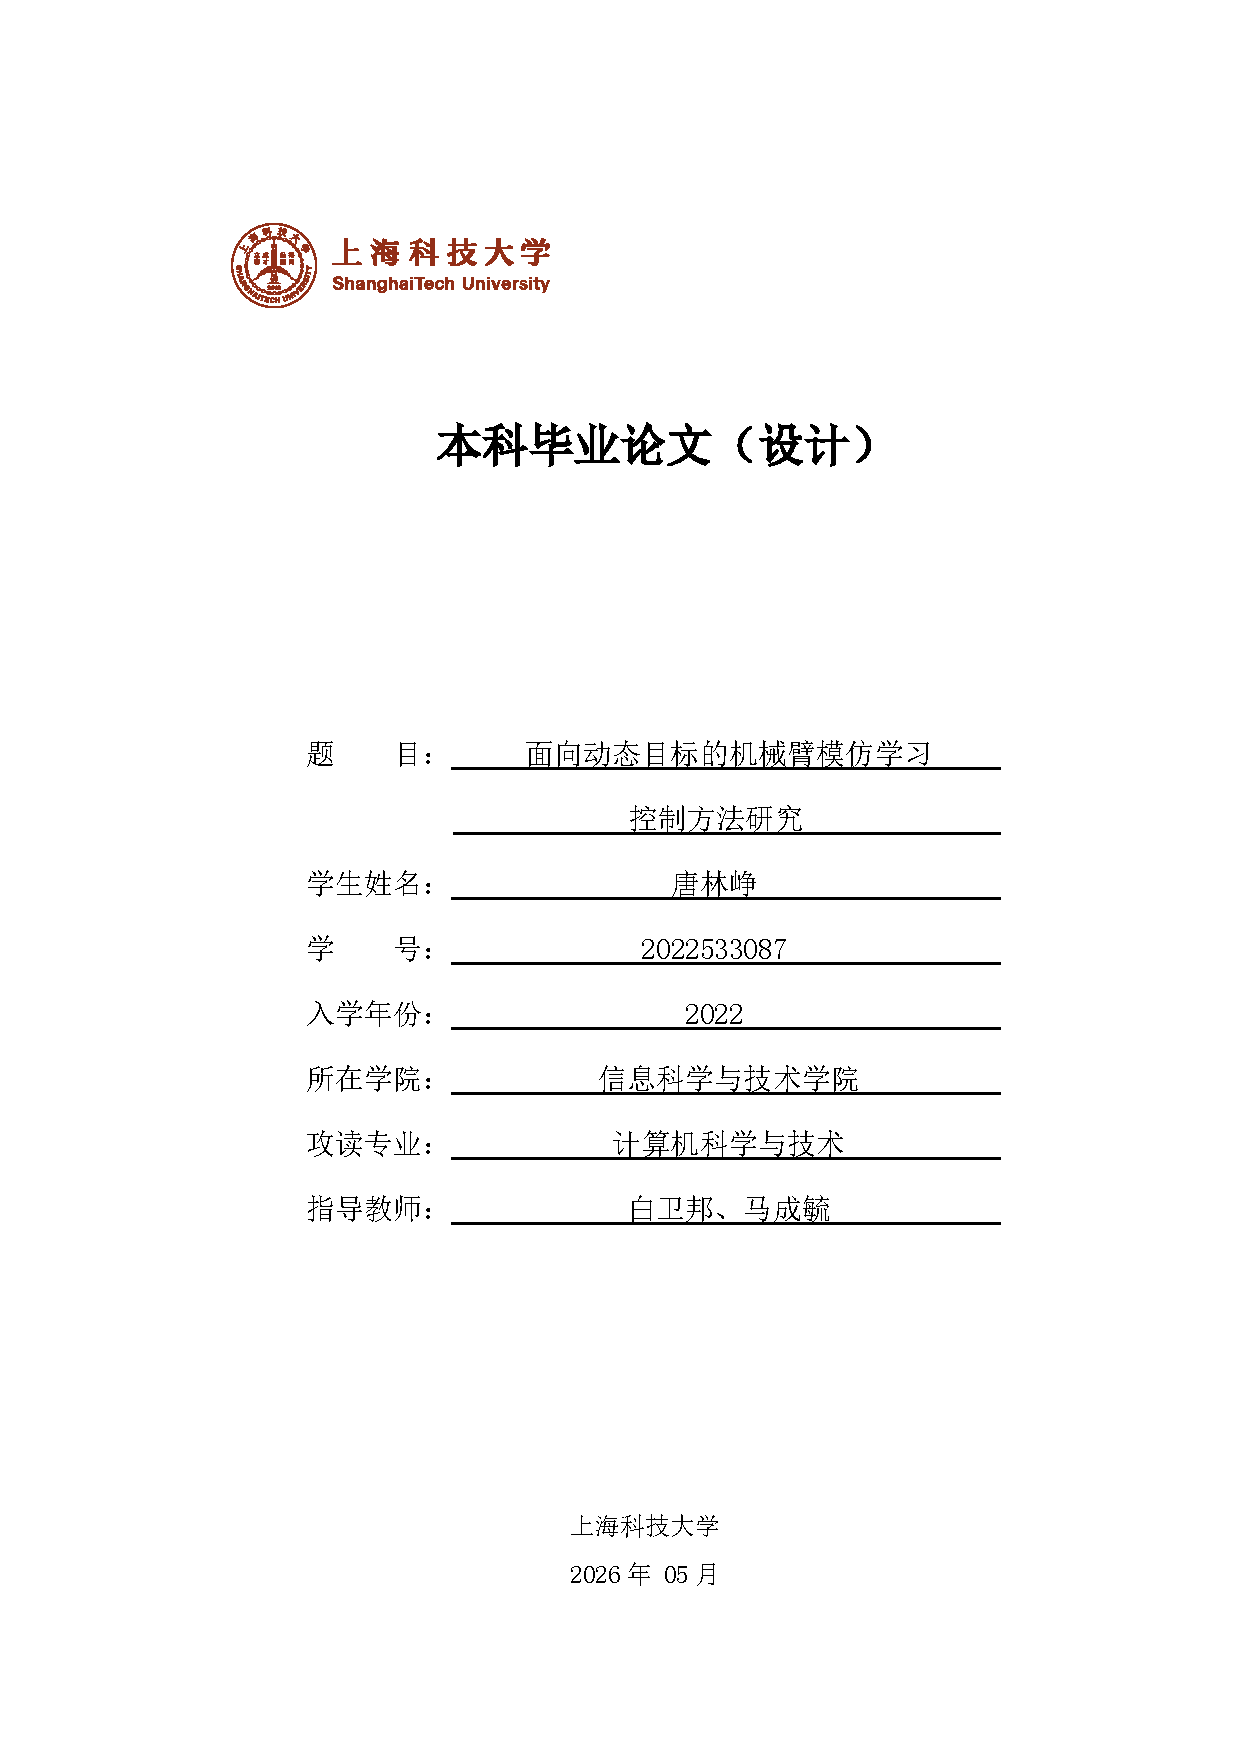
\includepdf[pages=-]{cover.pdf}% 插入预生成的封面PDF（中文+英文）
%-
%-> 作者声明
%-

\includepdf[pages=-]{integrity.pdf}% 插入预生成的诚信书

\includepdf[pages=-]{copyright.pdf}% 插入预生成的版权授权书
%-
%-> 中文摘要
%-
\chapter*{摘\quad 要}\chaptermark{摘\quad 要}% 摘要标题
\setcounter{page}{1}% 开始页码
\pagenumbering{Roman}% 页码符号

动态目标抓取要求机械臂在目标持续平移和旋转时，依次完成接近、相对位姿对齐、夹爪闭合、保持与搬运。与静态抓取或单步轨迹跟踪相比，该任务对运动目标的相对表示、短时历史信息的利用以及闭环时机的判断有较高要求。本文以动态立方体抓取为研究对象，构建目标中心动作块模仿学习框架，并在统一数据、统一动作接口和统一闭环执行协议下比较多类学习策略。研究重点不在于提出单一新模型，而在于分析哪些设计因素真正决定动态目标抓取的闭环成功率。

本文收集了5000条成功专家示教，并在每个主要条件下进行750回合闭环评估，得出了三个主要发现。

第一，目标中心表示是最稳定的性能决定因素。以ACT为例：使用目标中心表示时成功率为57.3\%--59.2\%；切换至世界坐标表示后降至8.8\%--27.2\%，性能差距约30--50个百分点。这一差距明显大于ACT与BC-RNN之间的架构差异（约10个百分点）。

第二，当物体姿态随机变化且伴随平移时，策略需要时间结构和动作块输出。单步BC几乎完全失败（0.1\%），而BC-RNN和ACT分别达到48.7\%和59.2\%。这表明抓取面选择、姿态对齐和闭合时机的判断依赖于历史上下文和多步动作组织。

第三，单纯依靠增加模型容量或更换策略类别并不能保证成功。在本文采用的低维动作空间与10步DDIM条件下，扩散策略（DP）在不同模型容量下的成功率均在1.3\%--2.8\%之间。这表明动态抓取性能主要取决于表示和时间结构，而非模型复杂度。

除表示和时间结构外，感知噪声下的状态估计方式同样影响闭环表现。噪声实验表明，状态估计策略需要与控制器结构适配。专家FSM-MPC控制器在强噪声下完全失效（0.0\%），加入卡尔曼滤波后恢复至56.4\%，说明显式状态估计对基于规则和优化的控制器至关重要。相比之下，ACT和BC-RNN在卡尔曼滤波后的变化仅为$+2.5$和$-5.2$个百分点，表明学习策略依靠历史窗口和动作块结构已自然具备隐式时间平滑能力。综合来看，在FSM-MPC专家示教框架内，动态目标抓取的有效学习控制取决于目标中心表示、时间动作块与状态估计方式三者的协调，而非单纯更换或扩大策略架构。上述发现表明，学习策略的表示设计与经典控制器的状态估计之间存在互补关系，体现了混合控制的基本思路。

\keywords{模仿学习，动作块，动态目标抓取，目标中心表示，混合控制}% 中文关键词
%-
%-> 英文摘要
%-
\chapter*{Abstract}\chaptermark{Abstract}% 摘要标题

Dynamic object grasping requires a manipulator to approach, align with, close on, hold, and transport a target that is continuously moving. Compared with static grasping or one-step trajectory tracking, this task demands accurate relative-motion representation, short-horizon temporal context, and precise timing of gripper closure within the closed loop. This thesis studies dynamic cube grasping through a target-centric action-chunk imitation learning framework, where multiple learned policies are compared under the same demonstration dataset, action interface, and closed-loop execution protocol. The goal is not to propose a new architecture, but to identify which design factors determine closed-loop success in moving-target manipulation.

Based on 5000 successful expert demonstrations and 750 closed-loop evaluation episodes per main condition, the experiments yield three main findings.

First, target-centric representation is the most consistent performance determinant. ACT reaches 57.3--59.2\% success with target-centric state, but drops to 8.8--27.2\% with world-frame state. This gap of roughly 30--50 percentage points far exceeds the architectural difference between ACT and BC-RNN (roughly 10 percentage points).

Second, when the object undergoes arbitrary tumbling and translation, temporal structure and action chunks are essential. One-step BC almost completely fails (0.1\%), whereas BC-RNN and ACT reach 48.7\% and 59.2\% respectively. This indicates that history and multi-step action organization are necessary for grasp-face selection, pose alignment, and gripper closing timing.

Third, model class or capacity alone does not ensure success. Under the low-dimensional action space and 10-step DDIM setup used in this thesis, all DP variants remain in the 1.3--2.8\% success range, suggesting that representation and temporal structure are stronger constraints than model scale in this setting.

The noise experiments further show that state estimation must be aligned with the controller structure. The expert FSM-MPC controller fails completely under strong perceptual noise (0.0\%), but recovers to 56.4\% with a Kalman filter, indicating that explicit state estimation is critical for rule- and optimization-based control. In contrast, ACT and BC-RNN exhibit only modest shifts of +2.5 and -5.2 percentage points with Kalman filtering, suggesting that learned temporal policies already provide inherent smoothing through history windows and action chunks.

Overall, effective learned control for dynamic grasping depends on three coordinated elements: target-centric representation, temporal action chunks, and controller-appropriate state estimation. These design factors, rather than policy architecture scaling, determine success within the FSM-MPC expert demonstration framework. This thesis demonstrates a hybrid control perspective in which learned policies and classical controllers are complementary.

\englishkeywords{Imitation Learning, Action Chunking, Dynamic Grasping, Target-Centric Representation, Hybrid Control}% 英文关键词
%---------------------------------------------------------------------------%
% title page, abstract, dedication
{% content list region
\linespread{1.2}% local line space
%\intotoc{\contentsname}% add link to contents table and bookmark
\tableofcontents% contents catalog
%\intotoc{\listfigurename}% add link to contents table and bookmark
%\listoffigures% figures catalog
%\intotoc{\listtablename}% add link to contents table and bookmark
%\listoftables% tables catalog
}
%-
%-> Mainmatter
%-
\mainmatter% initialize the environment
%---------------------------------------------------------------------------%
%->> Main content
%---------------------------------------------------------------------------%
\chapter{引言}\label{chap:introduction}

\section{研究背景}

考虑如下场景：分拣传送带上，立方体零件持续平移和旋转，机械臂需逐一抓取并将其搬运至指定目标区域。与”传送带停止—抓取—启动”的间歇模式不同，动态抓取要求机械臂在目标运动过程中依次完成两项任务：其一，接近目标并实现相对位姿对齐；其二，在恰当时机闭合夹爪，保持抓取并搬运至指定区域\citep{marturi2019dynamic,zhang2022robotic,newbury2023deep}。机械臂需要跟踪当前目标位置、预测目标短期运动，同时可靠地判断当前任务阶段——夹爪闭合过早会导致对齐不足，闭合过晚则可能错过可达窗口。

现有的动态抓取方法大致分为两类。基于模型的方法（如FSM-MPC）能够显式处理位置、姿态、平滑性约束和执行约束，在状态观测准确时结构清晰、可解释性强\citep{rawlings2017model,nubert2020safe}。然而，目标位姿观测存在噪声、离群点或时延时，手工阶段规则和参考轨迹构造会将感知误差直接传递至控制输出，导致阶段判定和跟踪参考系统性地偏离真实状态。另一方面，模仿学习从专家示教中学习动态追踪、相对位姿对齐和夹爪闭合时机\citep{argall2009survey}，但离线策略在闭环执行时会受到分布偏移和误差累积的影响\citep{ross2010efficient,ross2011reduction}。

上述两类方法各有优劣，但更根本的问题在于：策略架构、观测噪声、状态估计策略和执行器选择等因素相互纠缠，闭环成功率的差异究竟源自何处？已有工作中，这些因素通常随输入输出表示和执行协议的不同而变化，彼此难以解耦，因此各因素的独立贡献无法被单独衡量。

本文构建了统一的实验框架，系统分析了影响动态抓取闭环成功率的关键因素。该框架的核心是统一的目标中心动作块模仿学习接口，使所有策略共享相同的观测--动作表示、运行时阶段约束和MPC跟踪执行器。基于该框架，本文以大规模专家示教为基础，比较了BC、BC-RNN、ACT和DP四类策略。

\section{相关工作}
\label{sec:related-work}

\subsection{动态目标抓取}

动态目标抓取要求机器人在目标持续运动过程中完成相对位姿对齐和接触决策，难度远高于静态抓取。现有抓取综述通常涵盖解析抓取、采样规划、学习抓取和闭环视觉伺服等路线，探讨实现鲁棒操作的不同技术路径\citep{zhang2022robotic,newbury2023deep}。目标运动时，机器人还需估计其运动趋势，在有限时间内确定接近路径、抓取面、夹爪朝向和闭合时机\citep{marturi2019dynamic,alshanoon2022robotic}。这意味着动态抓取需同时完成感知、预测、阶段判断与执行跟踪，而非仅依赖单帧抓取姿态估计。

传统动态抓取方法通常依赖几何预测、视觉跟踪、轨迹优化或显式状态机。状态观测准确且运动模型可用时，这类方法解释性强、稳定性好；但目标姿态、速度或感知噪声变化较大时，手工阶段规则和参考轨迹构造可能变得脆弱。

本文以翻滚场景（立方体初始姿态均匀随机、绕空间轴旋转）中的立方体抓取为核心任务，系统分析目标运动、姿态对齐和抓取阶段时机对闭环成功率的影响。专家FSM-MPC控制器同时作为示教生成器和对照基线：其一，检验基于模型的控制器在噪声观测条件下是否必须依赖显式状态估计；其二，检验学习策略能否通过隐式利用时间冗余形成另一种噪声鲁棒机制。

现有动态抓取研究往往使用不同的评估标准、执行器和观测表示，因此很难判断不同工作之间的性能差异，究竟是策略设计所致还是实验设置使然。本文以固定评估标准、共享观测--动作接口和受控消融设计，搭建了从感知到执行的完整比较框架。

完整的动态目标抓取包含两个相互关联但可分离的子问题：抓取点选择（在物体表面确定抓取位置和夹爪朝向）和轨迹跟踪与时机控制（在目标运动过程中完成接近、对准和闭合）。抓取合成研究从解析方法演进至基于学习的方法，已成为独立的技术方向\citep{bohg2014grasp,newbury2023deep,morrison2018ggcnn,mahler2017dexnet}；拦截抓取问题的早期工作则从模型预测和控制角度处理运动目标的跟踪与抓取\citep{allen1993automated}。本文聚焦于后者——在给定抓取点（立方体中心，从上方抓取）的条件下，研究目标中心表示、时间动作块结构和噪声鲁棒性策略对闭环成功率的影响。本文有意将研究范围限定于该设定：固定抓取点后，实验比较可以更清晰地分离表示、时序结构和执行器因素的效应，而不受抓取点选择变化的干扰。这一设计选择的局限性与泛化范围将在第五章进一步讨论。

\subsection{模仿学习与闭环分布偏移}

模仿学习通过专家示教学习从观测到动作的映射，是机器人操作中常用的数据驱动策略学习方法\citep{argall2009survey}。行为克隆将专家轨迹分解为监督学习样本，这一思想可追溯到端到端驾驶策略ALVINN\citep{pomerleau1989alvinn}。但离线训练策略的动作会在闭环执行中改变后续观测分布；一旦进入训练数据未能覆盖的分布外状态，误差可能随时间累积并导致任务失败\citep{ross2010efficient,ross2011reduction}。动态抓取尤其容易出现这类问题，因为轻微的相对位姿误差会改变后续可抓取窗口和夹爪闭合时机。

交互式数据聚合和更大规模示教可以缓解分布偏移\citep{ross2011reduction,mandlekar2021matters}，但本文使用算法生成的离线专家示教，因此更聚焦于结构设计对闭环执行的影响。本文将单步BC作为基础参照。若单步回归在翻滚场景中即可成功，则说明目标中心表示和监督信号已足够应对该任务；此时闭环分布偏移的缓解应归因于历史条件窗口、动作块重规划和阶段约束的组合，而非数据聚合。

现有离线模仿学习研究在策略比较中，通常由于观测表示、动作空间和执行协议不一致，难以分离架构效应与实验设置效应。举例来说，观测表示的变化给同一策略带来的性能波动，可能比同一表示下不同策略之间的差异更大。本文要求所有策略共享相同的观测--动作接口和运行时结构，将表示效应、架构效应和执行器效应分离为独立消融维度，进而量化各因素的相对贡献。

\subsection{时间建模与动作分块}

时间建模是动态操作任务中的关键设计。循环网络通过隐藏状态整合历史观测，在部分可观测、多阶段操作或示教质量变化的任务中构成了强基线\citep{mandlekar2021matters}。BC-RNN通常使用GRU或LSTM编码历史信息，让策略能够利用目标速度、相对相位和近期执行误差等时序线索。在动态抓取任务中，这些线索直接关系到抓取面选择、对齐阶段持续时间和夹爪闭合时机。

动作分块进一步将策略输出从单步动作扩展为短时动作序列。ACT将机器人操作策略建模为条件动作序列生成问题，利用Transformer编码和条件序列生成提高闭环动作的时序一致性\citep{zhao2023learning,vaswani2017attention}。在本文框架内，BC、BC-RNN、ACT和DP都输出32步任务空间动作块，并在运行时每16步重规划一次，因此结果差异并非源自动作块接口的有无。本文关注的核心问题是：在统一动作块接口和翻滚场景条件下，循环结构、Transformer-CVAE结构和扩散去噪结构的相对性能差异。为此，本文在该场景中开展历史长度消融，检验更长历史窗口是否对循环和Transformer策略持续有益，抑或存在收益边界。

现有时间策略比较中有一个问题尚未解决：ACT的原始论文报告其性能优于BC-RNN，但该工作使用了不同的观测表示和执行设置；因此无法确定ACT的增益来自Transformer-CVAE架构、动作块结构还是表示选择。本文基于统一表示和接口，直接比较不同时间机制（GRU循环、Transformer注意力、扩散去噪）的闭环表现。这一设计使时间结构成为唯一变量，从而分离时间机制的独立效应。

\subsection{生成式动作策略与扩散策略}

机器人操作中的动作分布通常呈现多模态特性：在相同观测下，可能存在多种可行的接近方向、抓取面或闭合时机。混合密度模型、能量模型和生成式模型都曾用于刻画这类一对多映射\citep{bishop1994mixture,florence2022implicit}。扩散模型通过逐步加噪和反向去噪学习数据分布\citep{ho2020denoising,song2021denoising}，扩散策略（DP）则将这一思想应用于机器人动作序列生成，在视觉操作任务中展现了较强的轨迹生成能力\citep{chi2023diffusion}。

生成式动作建模本身并不确保更高的闭环成功率。DP的闭环表现受多种设计因素影响，包括状态表示、动作参数化、模型容量、采样步数和跟踪执行器等。本文在低维目标中心任务空间接口中比较DP与确定性动作块策略，同时检验DP在不同容量和世界坐标表示下的表现。此外，本文还检验了验证噪声预测损失是否可作为闭环成功率的替代指标。通过比较验证损失与闭环成功率的变化趋势，本文将生成式建模能力与其在闭环控制中的实际收益加以区分——更低的验证损失并不保证更高的闭环成功率。

现有扩散策略研究通常同时报告验证损失和闭环成功率，但尚未系统检验二者之间的相关性——更低的验证损失是否对应更高的闭环成功率。原始Diffusion Policy研究虽报告了不同容量和表示配置下的结果，但并未围绕验证损失与闭环成功率的关系开展受控分析。此外，扩散模型在机器人操作中的应用并不限于动作分块去噪——Diffuser等方法在轨迹级别实施扩散规划\citep{janner2022diffuser}，其设计和接口选择不同于DP。本文的DP实验基于固定推理步数的条件扩散去噪实现，因此相关结论仅限于该特定配置下的表现，不推广至其他扩散策略变体。本文在同一框架内系统改变DP容量（1.5M至18M）和表示（目标中心与世界坐标），直接检验验证损失与闭环成功率之间是否存在单调关系。

\subsection{目标中心表示与相对动作}

机器人操作中的坐标表示显著影响学习难度。若直接在世界坐标系中学习末端位姿参考，同一种抓取意图会随目标位置和姿态变化而产生数值差异很大的动作目标；而在目标或物体坐标系中表示动作，策略可以直接学习”相对目标如何接近、对齐和闭合”。类似的相对轨迹或物体中心表示已被用来提高机器人操作策略对空间变化的泛化能力\citep{zeng2021transporter,chi2024universal}。

本文将历史观测、未来目标条件和动作标签均表示于目标中心坐标系。通过系统比较目标中心表示与世界坐标表示（各含完整和紧凑两种变体），直接量化表示选择对闭环成功率的影响。关键问题是：表示选择与架构选择，究竟哪一个对闭环成功率的影响更大？如果目标中心与世界坐标之间的成功率差距超过BC与ACT之间的差距，则说明在动态抓取任务中，表示设计比模型选择更为根本。

已有研究分别证实了目标中心表示的有效性和特定架构的优越性，但尚未在同一实验中同时量化两者的影响程度并直接比较。本文通过交叉表示类型与策略类型的全因子实验设计补充了这一缺失：在统一评估协议下同时报告表示效应与架构效应及其95\% Wilson置信区间，读者可以直接比较两类设计选择的相对重要性，无需依赖不同实验设置的结果来推断。

\subsection{混合控制与跟踪执行器}

学习策略直接输出关节命令可以减少对手工结构的依赖，但接触约束、相位逻辑和低层跟踪也因此完全交由数据驱动模型来习得。分层模仿学习和学习规划器方法通常将任务意图、局部轨迹和低层执行分开建模\citep{lynch2020learning,mandlekar2020iris,wang2023mimicplay}。本文借鉴类似思想，但低层执行仍由结构化跟踪执行器负责：学习策略预测任务空间动作块，FSM约束阶段推进，MPC跟踪执行器负责跟踪任务空间参考。这一设计确保策略比较主要反映动作块生成质量，而非执行器的差异。

现有混合控制框架通常将学习策略与固定执行器绑定评估，很少在同一实验中控制执行器差异。因此，不同策略采用不同执行器时，性能差异同时反映策略设计和执行器能力，因而难以归因。本文主实验统一使用MPC跟踪执行器，与专家结构保持一致，从而将执行器差异从策略架构比较中剔除。综上，本文后续章节基于统一的观测--动作接口和运行时结构，将表示效应、架构效应和执行器效应分离为独立消融维度，以系统回答前述文献中尚未解决的问题。

\section{研究问题}

本文以翻滚环境为主要实验平台：立方体初始姿态均匀随机，绕空间轴以中等角速度旋转并同时平移。本文中”翻滚”指三维姿态绕非固定竖直轴变化，而非立方体与地面接触滚动。同时，本文在较简单的定轴自旋场景（立方体初始姿态固定、绕$z$轴自旋）中进行对照评估，以确认翻滚场景中的性能下降源于任务难度，而非评估协议或场景设定差异（详见第四章\S\ref{sec:main-clean}）。

基于上述设置，本文聚焦三个核心问题：

\begin{enumerate}
    \item 表示选择：目标中心表示是否优于世界坐标表示——更重要的是，这一影响是否超过架构选择？已有工作通常预设某一坐标表示，但很少将其作为独立变量进行消融研究。本文在目标中心表示（完整和紧凑）与世界坐标表示（完整和紧凑）之间直接比较，检验表示选择对BC和ACT的影响程度。
    \item 时间结构：翻滚场景是否需要超越单步回归的时间结构，且历史窗口长度如何影响循环和注意力策略？该场景的难点在于随机初始姿态和空间轴旋转使抓取面选择和姿态对齐变得复杂。本文以单步BC检验时序信息的必要性，以BC-RNN和ACT检验循环编码和Transformer查询能否弥补这一缺陷，并通过历史长度消融分析时间上下文的收益边界。
    \item 噪声鲁棒性：应通过显式状态滤波实现，还是依赖策略自身的隐式时间冗余利用？本文分别检验专家FSM-MPC控制器和学习策略在引入卡尔曼滤波后的表现，以区分显式状态估计和隐式时间冗余利用在动态抓取中的互补角色。
\end{enumerate}

\section{方法概述与主要贡献}

本文采用由学习规划器和结构化跟踪执行器组成的混合控制框架，如图\ref{fig:intro-overview}所示。由有限状态机和MPC组成的专家控制器首先生成成功示教，学习策略随后基于目标中心历史观测和短时未来目标条件预测32步任务空间相对动作块。在线执行时，系统每16步重新规划一次，并由单调相位状态机与MPC跟踪执行器共同完成阶段推进和轨迹跟踪。

本文的主要贡献有三：

\begin{enumerate}
    \item 构建动态立方体抓取实验框架。以翻滚场景为主要设置、定轴自旋场景为验证对照，以闭环成功率为核心评估指标（每条件750回合），覆盖无噪观测和强噪声观测两种条件。
    \item 提出统一的目标中心动作块模仿学习接口。该接口使BC、BC-RNN、ACT和DP共享输入输出表示、阶段约束和评估标准，从而将架构差异与表示差异和执行器差异解耦。
    \item 在以FSM-MPC为专家的实验框架内，系统实验明确了决定动态抓取闭环成功率的三个关键因素。其一，目标中心表示带来的提升最为稳定——在翻滚场景中，表示选择造成的成功率差距超过了架构选择的差距。其二，时间结构策略（BC-RNN、ACT）显著提高了翻滚场景中的闭环成功率。其三，噪声鲁棒性存在两条互补路径：显式状态滤波对模型控制器不可或缺，隐式时间冗余利用对学习策略已足够。
\end{enumerate}

\begin{figure}[!htbp]
    \centering
    
\includegraphics[width=0.95\textwidth]{fig_intro_overview}
    \caption{目标中心动作块模仿学习框架。专家示教由FSM+MPC控制器生成，学习策略基于目标中心表示预测任务空间动作块，运行时通过单调相位状态机和MPC跟踪执行器实现闭环控制。}
    \label{fig:intro-overview}
\end{figure}

\section{章节安排}

本文其余章节安排如下。

第二章介绍动态抓取任务设置与专家控制器：涵盖仿真平台与评估协议，定轴自旋和翻滚两个实验场景的定义与设计意图，FSM-MPC专家架构与五阶段逻辑，以及专家示教数据集的采集与筛选。

第三章介绍统一模仿学习策略与实验设计：涵盖目标中心表示与动作块构造，BC、BC-RNN、ACT和DP四类策略的统一接口与训练协议，以及闭环执行与评估标准。

第四章报告实验结果：以定轴自旋和翻滚场景的双场景对比为主线，依次分析无噪观测下的跨场景策略比较、观测表示与历史结构消融、噪声鲁棒性与状态估计、时间集成消融，以及数据规模与模型容量边界。

第五章总结全文，讨论研究局限并展望未来工作。

\chapter{动态抓取任务与专家控制器}\label{chap:task-expert}

\section{任务设置}

本文使用Genesis仿真平台构建动态立方体抓取任务\citep{genesis2024}。场景包含固定基座的Franka Research 3七自由度机械臂、Franka Hand二指夹爪\citep{franka2026research3,franka2026hand}和一个边长$0.05\,\mathrm{m}$的立方体。每个回合开始前，立方体在预设空间区域内随机生成，并以给定的线速度和角速度开始运动。机械臂需依次完成五个阶段——接近、对齐、闭合抓取、保持和搬运——最终将立方体送入目标区域。仿真步长为$\Delta t=0.01\,\mathrm{s}$；每个回合最多运行2400个仿真步。

任务目标是将立方体运送至半径$0.10\,\mathrm{m}$的目标区域内；本文以立方体中心到目标中心距离不超过$0.05\,\mathrm{m}$作为成功判据，达到该条件时记为成功回合。本文以闭环成功率为主指标，即成功回合数除以总评估回合数。主实验中，每个策略与场景组合均评估750个闭环回合。

\begin{figure}[!htbp]
    \centering
    
\includegraphics[width=0.90\textwidth]{fig_task_setup}
    \caption{Genesis仿真平台中的FR3与Franka Hand动态立方体抓取任务。图中展示立方体生成区域和目标区域。}
    \label{fig:task-setup}
\end{figure}

\section{实验场景}\label{sec:experiment-scenes}

本文设置两个实验场景：定轴自旋场景（立方体姿态固定，仅绕$z$轴自旋）和翻滚场景（立方体初始姿态均匀随机，绕空间轴旋转）。两个场景的生成区域、线速度范围、机械臂配置和成功判据完全一致，关键区别在于抓取面是否预先确定：定轴自旋场景中抓取面固定且已知；翻滚场景中抓取面需在执行过程中动态确定。

两个场景的目的不同。定轴自旋场景是验证基线：由于抓取面固定且已知，该场景用于确认策略具备基本的轨迹跟踪和时序判断能力，为分析翻滚场景提供参照。翻滚场景是主实验场景：抓取面选择、姿态对齐和闭合时机判断在此才构成真实挑战——这正是本文研究问题的核心。

\subsection{定轴自旋场景}

立方体初始姿态固定（与世界坐标系原点姿态一致），绕世界坐标系$z$轴以$30$--$60\,\mathrm{deg/s}$的角速度自旋。线速度在$[-0.10,-0.10,-0.02]$到$[0.10,0.10,0.02]\,\mathrm{m/s}$的三维盒形范围内均匀采样，生成位置范围为$[0.20,-0.45,0.20]$到$[0.48,0.45,0.40]\,\mathrm{m}$。该场景中，控制器可预先确定抓取面，任务难点主要是轨迹跟踪和闭合时机判断。

\subsection{翻滚场景}

立方体初始姿态均匀随机（四元数在$\mathbb{S}^3$上均匀采样），绕空间轴以$15\,\mathrm{deg/s}$的角速度旋转。本文中”翻滚”指立方体绕空间轴旋转（初始姿态随机），并非物体在地面上接触滚动。线速度在$[-0.075,-0.075,-0.02]$到$[0.075,0.075,0.02]\,\mathrm{m/s}$的三维盒形范围内均匀采样，生成位置范围与定轴自旋场景相同。翻滚场景的核心挑战不在于自旋速度——其角速度$15\,\mathrm{deg/s}$甚至低于定轴场景的$30$--$60\,\mathrm{deg/s}$。真正的难度来自随机初始姿态和空间轴旋转的叠加：抓取面选择、姿态对齐和闭合时机判断这三个挑战相互耦合，是翻滚场景的核心难点。

综上，定轴自旋与翻滚场景构成由简至繁的两层测试环境。两个场景各采集5000条成功专家示教，共享相同的数据预处理流程（筛选、采样步幅、验证集比例等详见\S\ref{sec:expert-demos}）。

图~\ref{fig:ch2-scene-motion-snapshots}用同一相机视角展示两类场景中的立方体运动。为清晰展示立方体运动趋势，图中固定了起始位置并采用各场景允许的最大线速度与最大角速度。定轴自旋场景从固定初始姿态出发，抓取面不随回合变化；翻滚场景从随机初始姿态出发并绕空间轴旋转，姿态和可达抓取面随时间共同变化。

\begin{figure}[!htbp]
    \centering
    \captionsetup[subfigure]{font=footnotesize,skip=2pt}
    \begin{subfigure}[t]{0.31\textwidth}
        
\includegraphics[width=\linewidth]{fig_ch2_scene_motion_0_0}
        \caption{定轴自旋，$t=0.0\,\mathrm{s}$}
    \end{subfigure}\hfill
    \begin{subfigure}[t]{0.31\textwidth}
        
\includegraphics[width=\linewidth]{fig_ch2_scene_motion_0_1}
        \caption{定轴自旋，$t=0.8\,\mathrm{s}$}
    \end{subfigure}\hfill
    \begin{subfigure}[t]{0.31\textwidth}
        
\includegraphics[width=\linewidth]{fig_ch2_scene_motion_0_2}
        \caption{定轴自旋，$t=1.6\,\mathrm{s}$}
    \end{subfigure}

    \vspace{0.45em}
    \begin{subfigure}[t]{0.31\textwidth}
        
\includegraphics[width=\linewidth]{fig_ch2_scene_motion_1_0}
        \caption{翻滚，$t=0.0\,\mathrm{s}$}
    \end{subfigure}\hfill
    \begin{subfigure}[t]{0.31\textwidth}
        
\includegraphics[width=\linewidth]{fig_ch2_scene_motion_1_1}
        \caption{翻滚，$t=0.8\,\mathrm{s}$}
    \end{subfigure}\hfill
    \begin{subfigure}[t]{0.31\textwidth}
        
\includegraphics[width=\linewidth]{fig_ch2_scene_motion_1_2}
        \caption{翻滚，$t=1.6\,\mathrm{s}$}
    \end{subfigure}
    \caption{定轴自旋与翻滚场景的运动快照。上排为定轴自旋场景，下排为翻滚场景；三列对应同一回合中的三个时间点。}
    \label{fig:ch2-scene-motion-snapshots}
\end{figure}

\section{专家策略与示教采集}\label{sec:expert-demos}

专家策略由有限状态机（FSM）和MPC组成，包含五个阶段：(1)~接近阶段——根据预测的未来立方体姿态选择可达抓取面并移动至预抓取位姿；(2)~对齐阶段——持续跟踪短时抓取参考，待相对位姿误差满足闭合条件后转入闭合；(3)~闭合阶段——按固定时长闭合夹爪；(4)~保持阶段——维持抓取稳定；(5)~搬运阶段——将已抓取立方体运送至目标区域。FSM负责阶段切换、抓取时机和几何参考构造，MPC负责带约束的任务空间跟踪。

该专家既定义了示教分布，也作为第四章中模型控制方法的对比基线。本节从任务执行角度说明专家控制器的工作机制。专家控制器在每个回合开始时，根据当前末端状态和立方体真实状态生成一次抓取计划。计划使用$4.0\,\mathrm{s}$预测窗口，将时间分配给接近、对齐和闭合三个抓取相关阶段：对齐和闭合的预设时长分别为$0.80\,\mathrm{s}$和$0.30\,\mathrm{s}$；接近阶段时长取$0.50\,\mathrm{s}$与可用时间的一半中的较大值。

抓取面从立方体六个面中选择：控制器先用当前线速度和角速度外推接近结束时的立方体位姿，再对每个候选面计算可达性和朝向评分，排除不可达面后，综合考虑机械臂工作空间、面法向朝向和目标速度方向选定。选定抓取面后，专家生成两个几何参考：抓取面法向外侧$0.08\,\mathrm{m}$处的预抓取位姿，以及更靠近物体中心（沿法向进入物体内部$0.035\,\mathrm{m}$）的抓取位姿。接近阶段到达预抓取位姿的判定阈值为$0.04\,\mathrm{m}$。

图~\ref{fig:ch2-mpc-case-snapshots}展示了一个成功回合的可视化快照序列，呈现了上述FSM-MPC逻辑的闭环执行流程。该回合来自翻滚场景，共执行237步（$2.37\,\mathrm{s}$）后达到目标区域。接近阶段首先选择抓取面，并沿预抓取参考逐步靠近目标；末端到预抓取位姿的误差满足阈值后，状态机进入对齐阶段。对齐阶段中，MPC使用短时预测轨迹继续降低末端与抓取参考的相对误差；闭合判据连续满足3步后，控制器转入闭合。随后系统确认抓取稳定，之后进入搬运阶段，最终将立方体送入目标区域。

\begin{figure}[!htbp]
    \centering
    \captionsetup[subfigure]{font=footnotesize,skip=2pt}
    \begin{subfigure}[t]{0.48\textwidth}
        
\includegraphics[width=\linewidth]{fig_ch2_mpc_case_00}
        \caption{初始}
    \end{subfigure}\hfill
    \begin{subfigure}[t]{0.48\textwidth}
        
\includegraphics[width=\linewidth]{fig_ch2_mpc_case_01}
        \caption{选择抓取面}
    \end{subfigure}

    \vspace{0.45em}
    \begin{subfigure}[t]{0.48\textwidth}
        
\includegraphics[width=\linewidth]{fig_ch2_mpc_case_02}
        \caption{接近20\%}
    \end{subfigure}\hfill
    \begin{subfigure}[t]{0.48\textwidth}
        
\includegraphics[width=\linewidth]{fig_ch2_mpc_case_03}
        \caption{接近40\%}
    \end{subfigure}

    \vspace{0.45em}
    \begin{subfigure}[t]{0.48\textwidth}
        
\includegraphics[width=\linewidth]{fig_ch2_mpc_case_04}
        \caption{接近60\%}
    \end{subfigure}\hfill
    \begin{subfigure}[t]{0.48\textwidth}
        
\includegraphics[width=\linewidth]{fig_ch2_mpc_case_05}
        \caption{接近80\%}
    \end{subfigure}

    \vspace{0.45em}
    \begin{subfigure}[t]{0.48\textwidth}
        
\includegraphics[width=\linewidth]{fig_ch2_mpc_case_06}
        \caption{进入对齐}
    \end{subfigure}\hfill
    \begin{subfigure}[t]{0.48\textwidth}
        
\includegraphics[width=\linewidth]{fig_ch2_mpc_case_07}
        \caption{对齐中}
    \end{subfigure}
    \caption{FSM-MPC专家控制器在一个成功翻滚回合中的快照序列。快照按照实际闭环时间排序，展示从抓取面选择、接近预抓取位姿、短时MPC对齐、夹爪闭合、保持检测到最终搬运的完整状态机行为。}
    \label{fig:ch2-mpc-case-snapshots}
\end{figure}

\begin{figure}[!htbp]
    \ContinuedFloat
    \centering
    \captionsetup[subfigure]{font=footnotesize,skip=2pt}
    \begin{subfigure}[t]{0.48\textwidth}
        
\includegraphics[width=\linewidth]{fig_ch2_mpc_case_08}
        \caption{闭合就绪}
    \end{subfigure}\hfill
    \begin{subfigure}[t]{0.48\textwidth}
        
\includegraphics[width=\linewidth]{fig_ch2_mpc_case_09}
        \caption{进入闭合}
    \end{subfigure}

    \vspace{0.45em}
    \begin{subfigure}[t]{0.48\textwidth}
        
\includegraphics[width=\linewidth]{fig_ch2_mpc_case_10}
        \caption{闭合中}
    \end{subfigure}\hfill
    \begin{subfigure}[t]{0.48\textwidth}
        
\includegraphics[width=\linewidth]{fig_ch2_mpc_case_11}
        \caption{进入保持}
    \end{subfigure}

    \vspace{0.45em}
    \begin{subfigure}[t]{0.48\textwidth}
        
\includegraphics[width=\linewidth]{fig_ch2_mpc_case_12}
        \caption{保持中}
    \end{subfigure}\hfill
    \begin{subfigure}[t]{0.48\textwidth}
        
\includegraphics[width=\linewidth]{fig_ch2_mpc_case_13}
        \caption{进入搬运}
    \end{subfigure}

    \vspace{0.45em}
    \begin{subfigure}[t]{0.48\textwidth}
        
\includegraphics[width=\linewidth]{fig_ch2_mpc_case_14}
        \caption{搬运中}
    \end{subfigure}\hfill
    \begin{subfigure}[t]{0.48\textwidth}
        
\includegraphics[width=\linewidth]{fig_ch2_mpc_case_15}
        \caption{成功终止}
    \end{subfigure}
    \caption{FSM-MPC专家控制器在一个成功翻滚回合中的快照序列（续）。}
\end{figure}

\begin{table}[!htbp]
    \caption{FSM-MPC专家控制器的阶段逻辑。}
    \label{tab:expert-fsm-logic}
    \centering
    \small
    \renewcommand{\arraystretch}{1.15}
    \newcommand{\PhaseCell}[2]{\begingroup\renewcommand{\arraystretch}{0.82}\begin{tabular}[t]{@{}l@{}}#1\\[-0.45ex]{\footnotesize\textup{(#2)}}\end{tabular}\endgroup}
    \begin{tabularx}{\textwidth}{>{\raggedright\arraybackslash}p{0.13\textwidth}YY>{\centering\arraybackslash}p{0.12\textwidth}}
        \hline
        阶段 & 参考构造 & 切换条件 & 夹爪命令 \\
        \hline
        接近 & 跟踪预测抓取面的预抓取位姿；姿态先对齐夹爪接近轴，再对齐面内切向；接近过程中加入碰撞规避位移。 & 末端到预抓取参考的距离小于$0.04\,\mathrm{m}$时转入对齐；若候选抓取面不可达且无法切换则终止。 & 打开 \\
        对齐 & 在MPC时域内预测立方体短时运动，生成由预抓取位姿平滑过渡至抓取位姿的参考轨迹。 & 至少等待10步；位置误差小于$0.025+0.15\|v_c\|+0.02\|\omega_c\|$且姿态误差小于0.18，并连续满足3次后转入闭合；超过300步未满足则终止。 & 打开 \\
        闭合 & 保持抓取位姿参考，并在$0.30\,\mathrm{s}$内逐步闭合夹爪。 & 闭合时长满足要求且夹爪已闭合后转入保持。 & 闭合 \\
        保持 & 保持抓取位姿和闭合夹爪，检测物体是否随末端稳定保持。 & 末端与立方体中心距离连续20步小于$0.040\,\mathrm{m}$后转入搬运；长时间不稳定则终止。 & 闭合 \\
        搬运 & 将已抓取物体运送至目标区域；姿态跟踪权重降低，以优先保证平移运输稳定。 & 环境成功条件满足或回合超时。 & 闭合 \\
        \hline
    \end{tabularx}
\end{table}

对齐阶段的位置误差阈值随物体运动速度自适应调整：物体运动较快时，放宽位置容限以避免错过闭合时机；静止或低速时则收紧阈值，确保对齐精度。

MPC在每个控制步内求解一个短时域滚动优化问题，将任务空间参考转化为关节动作。设当前关节角为$q_0$，预测时域为$H$，优化变量为未来关节序列$q_{1:H}$，末端正运动学给出位置$p(q_h)$和姿态$R(q_h)$，任务空间参考为$(p^r_h,R^r_h)$。优化问题如下：
\begin{equation}
    \begin{aligned}
    \min_{q_{1:H}} \quad
    \sum_{h=1}^{H}\Big(
    & w_p\|p(q_h)-p^r_h\|_2^2
    + w_R\|e_R(R(q_h),R^r_h)\|_2^2 \\
    & + w_s\|q_h-q_{h-1}\|_2^2
    + w_v\left\|\frac{q_h-q_{h-1}}{\Delta t}\right\|_2^2
    + J_{\mathrm{lim}}(q_h)
    \Big),
    \end{aligned}
    \label{eq:expert-mpc-objective}
\end{equation}
其中$e_R(\cdot)$为姿态误差向量，$J_{\mathrm{lim}}$为关节限位惩罚项。优化同时约束关节位置和单步关节速度。

MPC预测时域设为$H=10$步，位置跟踪权重$w_p=300$显著高于姿态权重$w_R=50$以优先保证末端定位精度，平滑项权重$w_s=5$用于抑制关节抖动；最大迭代次数设为100。将上一时刻优化解在时域上向前滚动一步，作为当前优化问题的初值。在搬运阶段，控制器降低姿态误差和平滑项权重，以优先保证平移运输稳定。若MPC未收敛，或非搬运阶段跟踪误差超过阈值，则舍弃该关节序列，改用任务空间逆运动学作为替代控制方案。

该FSM-MPC控制器作为专家策略，为模仿学习提供示教数据。原始示教从翻滚场景采集，筛选出5000条成功专家轨迹用于训练。定轴自旋场景同样采集5000条示教，用作第四章行为克隆（BC）和扩散策略（DP）的验证对照（\S\ref{sec:main-clean}）。

数据集仅保留成功回合，并进一步筛选抓取相关阶段；动作标签取自专家参考轨迹。数据按每4步采样一帧的方式构建训练窗口，验证集占比5\%，数据划分采用固定伪随机种子以保证可复现性。主实验中，翻滚场景包含约19.4万个训练窗口和约1.0万个验证窗口。

\chapter{统一模仿学习策略与实验设计}\label{chap:policy-design}

\section{目标中心表示与动作块构造}

实验中所有学习策略均作为任务空间动作块规划器运行，而非端到端关节控制器。每个监督样本包含历史观测窗口、未来目标条件和专家动作块。历史长度记为$H_o$，主实验设$H_o=16$；动作块长度为$H_a=32$；未来条件长度为$H_c=50$。运行时每次规划32步动作块，但只执行前16步后重新规划，因此执行窗口为$H_{\mathrm{exec}}=16$。

目标中心表示把抓取问题转化为相对目标的接近与对齐——不需要在世界坐标中记录绝对末端轨迹。设立方体位置和姿态为$(p^c_t,q^c_t)$，末端执行器位置和姿态为$(p^e_t,q^e_t)$，$R(q)$为四元数对应旋转矩阵\citep{shoemake1985animating}，则相对末端位置和姿态为
\begin{align}
    \tilde{p}^e_t &= R(q^c_t)^\top(p^e_t-p^c_t),\\
    \tilde{q}^e_t &= (q^c_t)^{-1}\otimes q^e_t .
    \label{eq:target-centric-observation}
\end{align}
未来目标条件为7维序列，包含相对位置变化$\Delta p(3)$和相对四元数$\Delta q(4)$，给出未来50步的立方体运动预测。常速度外推模型根据当前观测生成该序列：位置以当前线速度线性外推，姿态以当前角速度逐步积分；外推结果再经目标中心坐标变换转为相对变化量。该构造不直接读取仿真中的未来真值——在真实部署中，只要能从感知系统估计出目标的当前速度，即可用相同的常速度模型在线生成未来条件。在随机姿态翻滚平移场景中，该外推只是近似（空间轴旋转时角速度方向本身在演化），但为策略给出了合理的短时运动参考。动作标签为8维序列，包含相对任务空间目标位置3维、相对目标四元数4维和夹爪值1维。主表示使用完整目标中心历史观测，其历史维度为14；紧凑目标中心表示、紧凑世界坐标表示和完整世界坐标表示供表示消融配置使用。

策略输出的相对动作块在运行时解码为世界坐标任务空间参考。若第$k$步预测动作为$(\hat{p}^{rel}_{t,k},\hat{q}^{rel}_{t,k},\hat{g}_{t,k})$，则对应世界坐标参考为
\begin{align}
    \hat{p}^{r}_{t+k} &= p^c_{t+k}+R(q^c_{t+k})\hat{p}^{rel}_{t,k},\\
    \hat{q}^{r}_{t+k} &= q^c_{t+k}\otimes \hat{q}^{rel}_{t,k}.
    \label{eq:relative-action-decode}
\end{align}
连续夹爪通道参与训练监督，但闭环执行中的夹爪命令由状态机决定，以避免连续回归在开闭突变附近产生不稳定拖尾。

\section{模仿学习策略}

本文比较四类共享输入输出接口的模仿学习策略：行为克隆（BC, Behavior Cloning）、循环行为克隆（BC-RNN, Recurrent Behavior Cloning）、动作分块变换器（ACT, Action Chunking Transformer）和扩散策略（DP, Diffusion Policy）。四类策略的输入均为历史观测窗口$O_t$和未来目标条件$C_t$，输出均为长度为$H_a=32$的任务空间动作块$\hat{A}_t$。因此，本节中模型的差异主要源于条件编码方式、动作块生成主干和训练目标，而非不同的观测、动作定义或跟踪执行器。

\subsection{统一策略接口与辅助预测头}

每个策略输出包含三部分：连续动作块、闭合预测头和阶段预测头。连续动作块为$32\times 8$序列，其中位置、姿态通道在运行时解码为任务空间末端参考；连续夹爪通道参与监督训练，但闭环执行中的最终夹爪命令由状态机下达。闭合预测头预测夹爪闭合事件，触发从接近或对齐到闭合的切换；阶段预测头预测五类专家阶段，约束状态机单调推进。这一设计让四类学习模型均担当高层任务空间动作块规划器，而非直接输出关节命令。

图~\ref{fig:policy-architectures}展示四类策略在统一输入输出接口下的结构差异；表~\ref{tab:model-architecture-summary}列出各主模型的架构摘要。DP其余容量变体（1.5M、6M、18M）见附录。

\begin{figure}[!htbp]
    \centering
    
\includegraphics[width=0.95\textwidth]{fig_policy_architectures}
    \caption{统一动作块策略接口下的四类模仿学习模型。BC、BC-RNN、ACT和DP共享历史观测窗口、未来目标条件、32步任务空间动作块、闭合预测头和阶段预测头；差异主要源于条件编码方式、动作块生成主干和训练目标。}
    \label{fig:policy-architectures}
\end{figure}

\begin{table}[!htbp]
    \caption{模仿学习策略的主要架构设置。}
    \label{tab:model-architecture-summary}
    \centering
    \small
    \renewcommand{\arraystretch}{1.15}
    \begin{tabularx}{\textwidth}{>{\raggedright\arraybackslash}p{0.13\textwidth}>{\raggedright\arraybackslash}p{0.30\textwidth}Y}
        \hline
        策略 & 核心结构 & 主要设置 \\
        \hline
        BC & 历史因果1D-CNN、未来条件1D-CNN和MLP动作块回归头 & 历史通道$[64,128,192]$，未来通道$[64,128]$，条件维度192，MLP隐藏维度$[480,480,480]$ \\
        BC-RNN & GRU历史编码器、未来条件1D-CNN和GRU动作块解码器 & 条件维度192，2层GRU，隐藏维度218，约1.5M参数 \\
        ACT & 变换器编码器--解码器和CVAE后验编码器 & 变换器维度132，4头注意力，2层编码器、2层解码器，FFN维度544，隐变量维度32 \\
        DP 12M & 条件1D U-Net动作块去噪器 & 条件维度160，基础通道128，通道倍率$[1,2,4]$，100步训练扩散，10步DDIM推理 \\
        \hline
    \end{tabularx}
\end{table}

\subsection{确定性动作块策略：BC与BC-RNN}

BC是最简单直接的动作块回归基线。它以因果一维卷积编码历史观测，以一维卷积编码未来目标条件，再将两个条件向量拼接后送入MLP，一次性输出完整动作块。BC不包含显式循环状态，因此它主要检验目标中心表示和动作块接口本身是否足以完成动态抓取。

BC-RNN在BC的基础上加入循环时间结构。本文使用GRU而非LSTM作为循环单元\citep{cho2014learning,chung2014empirical}：GRU编码器读取经线性投影的历史观测序列，一维卷积编码未来条件，二者共同初始化GRU解码器。解码器以固定动作查询展开32步动作块，而非训练时读取专家上一动作、推理时读取自身上一预测的自回归结构。该设计避免了训练与推理之间动作输入分布的不一致，同时保持固定长度动作块接口；每16步重新规划时，新的闭环观测反馈自然进入策略。

\subsection{条件变分动作块策略：ACT}

ACT基于动作分块变换器的动作查询解码结构，以条件变分自编码器（CVAE）的隐变量建模动作块条件分布\citep{zhao2023learning,kingma2014autoencoding,sohn2015learning}。模型将历史观测和未来条件投影为带类型嵌入的序列标记，经变换器编码器形成上下文记忆；32个学习动作查询经变换器解码器一次性生成动作块。

训练时，ACT的后验编码器同时读取上下文记忆和专家动作块，输出隐变量分布$q_\phi(z|A^\ast,O,C)$的均值和方差，并经重参数化采样得到$z$。解码器接受该隐变量作为条件，生成动作块并同时预测闭合事件和阶段标签。推理时专家动作块不可用，模型取先验均值$z=0$，因此闭环执行仍是一次确定性前向传播。该结构的作用不是改变输入输出接口，而是在同一动作块接口下检验ACT的变换器条件建模和隐变量动作块分布是否能改善短时轨迹组织、阶段语义和闭合时机。

\subsection{生成式动作块策略：DP}

DP将动作块生成建模为条件去噪问题\citep{ho2020denoising,song2021denoising,chi2023diffusion}。给定专家动作块$A^\ast$，训练时先采样扩散步$s$和高斯噪声$\epsilon$，构造带噪动作块$A_s$；条件1D U-Net\citep{ronneberger2015unet}接收$A_s$、扩散时间嵌入以及从历史观测和未来条件导出的条件向量，预测噪声$\epsilon$。本文DP模型采用FiLM式条件残差块和U-Net下采样/上采样结构，并在去噪主干之外保留闭合和阶段辅助预测头。

推理时，DP从高斯噪声动作块开始，以10步DDIM确定性采样逐步生成32步动作块。相较于BC、BC-RNN和ACT的一次前向传播，DP需要多次去噪网络调用；但由于系统每16步才重新规划一次，其计算开销可被动作块执行窗口分摊。除主模型DP 12M外，另训练1.5M、6M和18M三个容量变体（见附录），以检验容量提升是否转化为闭环成功率增益。

\subsection{训练目标与检查点选择}

BC、BC-RNN和ACT的损失函数为动作$L_1$损失、闭合事件二分类交叉熵和阶段交叉熵的加权和：
\begin{equation}
    \mathcal{L}_{det}
    = \mathcal{L}_{action}
    + \lambda_c \mathcal{L}_{close}
    + \lambda_\phi \mathcal{L}_{phase}.
    \label{eq:deterministic-policy-loss}
\end{equation}
其中$\lambda_c=5.0$，$\lambda_\phi=1.0$。ACT额外加入KL正则项，KL权重为10.0，并设置10000步预热。DP以噪声预测损失为主损失，同时保留相同权重的闭合和阶段辅助监督：
\begin{equation}
    \mathcal{L}_{dp}
    = \mathbb{E}_{s,\epsilon}\|\epsilon_\theta(A_s,s,O,C)-\epsilon\|_2^2
    + \lambda_c \mathcal{L}_{close}
    + \lambda_\phi \mathcal{L}_{phase}.
    \label{eq:diffusion-policy-loss}
\end{equation}

所有主策略共享统一训练配置：使用AdamW优化器\citep{loshchilov2019decoupled}，学习率$2\times10^{-4}$，权重衰减$1\times10^{-6}$，共训练1500个轮次，bf16自动混合精度，启用TF32，EMA衰减为0.999。BC、BC-RNN和ACT按验证动作损失选择检查点；DP按验证噪声预测损失选择检查点。主实验中每个策略--场景--表示组合均采用固定随机种子；因此第四章报告的Wilson置信区间仅反映评估回合的抽样不确定性，不包含训练随机性的种子间方差。验证损失仅用于训练选择与优化诊断，第四章所有主要结论均以闭环成功率为准。

\section{闭环执行与跟踪执行器设置}

闭环执行时，学习策略每16个仿真步重新预测一个32步任务空间动作块。状态机单调推进，不允许阶段回退；闭合预测头可以触发从接近或对齐转入闭合，阶段预测头每步最多推进一个阶段。闭合阈值为0.5，滞回步数为5；转入保持或搬运后，夹爪保持闭合。若系统转入搬运或在保持中稳定10步，则控制切换为搬运控制。

主实验采用MPC跟踪执行器。学习策略输出的任务空间参考在抓取阶段由MPC跟踪器执行，MPC预测时域为10，位置、姿态和平滑权重分别为$w_{pos}=300$、$w_{orient}=50$、$w_{smooth}=5$。若MPC求解失败或非搬运阶段跟踪误差过大，系统以IK风格目标作为回退方案。该设置保持了专家和学习策略之间的执行结构一致性，使策略比较主要反映动作块生成质量。


\section{训练与评估标准}

本文考察两类训练设置：无噪声训练和在线观测噪声增强训练。无噪声训练策略训练时不添加观测噪声；在线观测噪声增强训练策略在训练时注入与噪声评估匹配的观测扰动，包括位置噪声0.03、姿态噪声$10\,\mathrm{deg}$、速度噪声0.02、角速度噪声$5\,\mathrm{deg}$、随机丢弃率0.05、漂移标准差0.01、离群点概率0.02、离群点幅度0.15和2帧时延。噪声评估环境叠加漂移、高斯噪声、离群点、随机丢弃和时延的组合扰动；随机姿态翻滚平移噪声场景通过独立噪声预设构造，不基于无噪观测设置手工修改。图~\ref{fig:ch3-observation-noise-trajectory}以一条真实示教轨迹为例，可视化该噪声栈对立方体位置观测的影响。

\begin{figure}[!htbp]
    \centering
    
\includegraphics[width=\textwidth]{fig_ch3_observation_noise_trajectory}
    \caption{无噪观测轨迹与噪声观测轨迹对比。左图在三维空间中叠加同一条立方体位置轨迹的无噪观测和噪声观测，黑色圆点和星号分别标记无噪轨迹的起点和终点，箭头表示运动方向，灰色连线表示部分时刻的观测偏移；线框立方体的一个角点位于坐标原点，其边长为5 cm，用于对比观测噪声与物体尺度。右图给出噪声观测相对无噪观测的位置误差随时间的变化，并标出离群点抽样和随机丢帧导致的陈旧观测。该图仅展示位置分量；训练和评估中的姿态、速度与角速度同样按本文噪声设置受到扰动。}
    \label{fig:ch3-observation-noise-trajectory}
\end{figure}

主评估使用750个闭环评估回合，并报告闭环成功率。记总回合数为$n$，成功回合数为$n_s$，则成功率点估计为$\hat{p}=n_s/n$。本文以95\% Wilson置信区间量化成功率的不确定性\citep{wilson1927probable}：
\begin{equation}
    \mathrm{CI}_\mathrm{Wilson} =
    \frac{\hat{p} + \frac{z^2}{2n} \pm z\sqrt{\frac{\hat{p}(1-\hat{p})}{n} + \frac{z^2}{4n^2}}}{1 + \frac{z^2}{n}},
    \quad z_{0.975}=1.96.
    \label{eq:wilson-ci}
\end{equation}
与Wald区间相比，Wilson区间在$\hat{p}$接近0或1时不会产生零宽度区间，因此即使策略成功率接近0\%或100\%，仍能给出合理的置信范围。750回合评估中，50\%成功率处的区间半宽约为$\pm3.6$个百分点，足以在多数实验条件间区分有意义的性能差异。300回合探索性评估的区间半宽约为$\pm5.7$个百分点，解读相应结果时需考虑这一较大的不确定性。

第四章的噪声鲁棒性分析涉及两类卡尔曼滤波实验：专家FSM-MPC控制器的强噪声评估，以及学习策略在滤波观测下的探索性评估。两类实验共用同一卡尔曼滤波器配置。滤波器作为感知前处理模块插入观测流：观测受到噪声损坏后，先经滤波器完成状态估计，再送入控制器或策略。

滤波器对立方体位置和线速度施加常速度过程模型的卡尔曼滤波\citep{kalman1960new}，过程噪声协方差参数为0.01。位置和速度的测量噪声参数分别设为0.03和0.02，与高斯抖动噪声的标准差一致。对于立方体姿态，滤波器采用指数平滑而非完整的卡尔曼滤波，平滑系数$\alpha=0.3$。该设计是工程上的折中：位置和速度的状态维度较低且动力学为线性，适合卡尔曼滤波；姿态的四元数流形上标准卡尔曼滤波需要更复杂的处理，指数平滑是轻量但有效的替代方案。

滤波后的观测替换原始噪声观测，但不改变下游策略或控制器的接口——滤波器和噪声注入模块都是感知层的组件，学习策略和专家控制器看到的始终是相同格式的观测向量。该滤波器配置同样应用于专家FSM-MPC的强噪声评估（第四章），以保证两类实验之间的可比性。

除主实验外，本文还通过受控消融研究各设计因素的影响。表示消融比较完整目标中心表示、紧凑目标中心表示、完整世界坐标表示和紧凑世界坐标表示；历史长度消融比较紧凑目标中心表示的不同$H_o$；数据量消融比较10\%、25\%、50\%和100\%数据；容量实验比较BC-RNN和DP扩容结果。所有验证损失仅用于训练选择与优化诊断，不能替代闭环性能。

\chapter{实验结果与分析}\label{chap:results}

本章以闭环成功率为主指标，报告动态抓取实验结果。除特别说明外，主表中的每个策略--环境组合均包含750个闭环评估回合。所有实验均在随机姿态翻滚平移场景中进行——立方体初始姿态均匀随机，绕空间轴以$15\,\mathrm{deg/s}$旋转并同时平移。为验证基线策略实现的正确性，在较简单的固定轴自旋平移场景中进行补充验证（详见\S\ref{sec:main-clean}）。本章的分析顺序与论文主线一致：首先比较无噪观测下的策略性能，然后分析目标中心表示，接着讨论噪声鲁棒性——包括在线观测噪声增强的收益与代价、专家FSM-MPC控制器的卡尔曼滤波评估、学习策略在显式状态估计下的表现，随后分析数据量、历史长度和模型容量边界。

\section{无噪观测下的策略比较}\label{sec:main-clean}

表~\ref{tab:main-clean-comparison}报告了四类策略的闭环成功率，图~\ref{fig:ch4-clean-main}以柱状图呈现相同数据。所有行均使用完整目标中心表示、历史长度16和MPC跟踪执行器。

\begin{table}[!htbp]
    \caption{主实验结果。所有结果均为750回合闭环成功率；方括号内为95\% Wilson置信区间。}
    \label{tab:main-clean-comparison}
    \centering
    \small
    \renewcommand{\arraystretch}{1.12}
    \begin{tabularx}{\textwidth}{>{\raggedright\arraybackslash}p{0.14\textwidth}ZZZZ}
        \hline
        策略 & BC & BC-RNN & ACT & DP 12M \\
        \hline
        闭环成功率 & \ResultCI{0.1\%}{[0.0, 0.8]} & \ResultCI{48.7\%}{[45.1, 52.2]} & \BestResultCI{59.2\%}{[55.6, 62.7]} & \ResultCI{2.5\%}{[1.6, 3.9]} \\
        \hline
    \end{tabularx}
\end{table}

\begin{figure}[!htbp]
    \centering
    
\includegraphics[width=0.85\textwidth]{fig_ch4_clean_main}
    \caption{主实验结果可视化。柱高为750回合闭环成功率，误差线为95\% Wilson置信区间。}
    \label{fig:ch4-clean-main}
\end{figure}

四类策略中，ACT的闭环成功率最高（59.2\%），其95\%置信区间[55.6, 62.7]与BC-RNN的[45.1, 52.2]不重叠，差异显著。BC-RNN的48.7\%远高于单步BC的0.1\% [0.0, 0.8]，说明GRU循环历史编码为策略提供了有效的时序上下文。BC几乎完全失败（750回合仅成功1次），可见单步前馈回归无法处理随机姿态翻滚平移所需的抓取面选择、姿态对齐和闭合时机判断。DP 12M仅2.5\% [1.6, 3.9]，在本文低维目标中心动作块接口、10步DDIM推理和固定噪声调度设置下未能将生成式建模能力转化为闭环成功率——此结论的范围限定参见\S\ref{sec:limitations}限制六；完整容量扩展和表示消融结果见附录\S\ref{sec:appendix-dp}。

为排除BC实现错误的可能性，本文以较简单的固定轴自旋平移场景（立方体初始姿态固定，绕$z$轴以$30$--$60\,\mathrm{deg/s}$自旋）补充评估了同一BC模型：其闭环成功率达45.7\% [42.2, 49.3]，确认BC实现正确，在随机姿态翻滚平移场景中的失效源自场景的内在难度而非代码错误。随机姿态翻滚平移的难点并不在于自旋速度（其角速度$15\,\mathrm{deg/s}$低于固定轴场景的$30$--$60\,\mathrm{deg/s}$），而在于初始姿态均匀随机和空间轴旋转使抓取面选择和姿态对齐变得复杂。

为排除DP实现错误的可能性，同一DP 12M模型在固定轴自旋平移场景中达41.9\% [38.4, 45.4]（附录表~\ref{tab:appendix-dp-scaling}），确认DP实现正确，在随机姿态翻滚平移场景中的低成功率同样源自场景的内在难度。

对失败回合的观察进一步印证了上述分析。从策略的失败评估轨迹中可归纳出三类典型失效模式。第一类是夹爪过早闭合：策略在末端执行器尚未充分到达抓取位置或姿态尚未对齐时即触发闭合，夹爪闭空后物体留在原处或被轻微碰偏——BC几乎全部失败属于此类，ACT和BC-RNN的剩余失败也以此为主。第二类是对齐阶段未对准或边缘碰撞：策略已接近物体，但闭合前夹爪的局部姿态未精确对准物体两侧，手指撞到边缘或角点将其推开或旋转脱出。第三类是阶段转换未完成的少数情况：策略未清晰地从接近转入闭合或搬运，夹爪保持打开、末端在物体附近徘徊，或阶段转换迟疑导致任务超时。

这三类失效模式从性质上印证了本文的两个核心设计动机：（a）闭合时机判断需要时序上下文——策略必须从历史观测中推断当前是否已对齐足够久、可以安全闭合；（b）相对姿态的精确对齐需要通过目标中心坐标来组织多步动作——这正是目标中心动作块接口设计的初衷。

\section{目标中心表示消融}

表~\ref{tab:representation-ablation}比较目标中心表示和世界坐标表示，图~\ref{fig:ch4-representation-ablation}以热力图展示表示差异的整体结构。本节直接检验本文方法的核心设计：策略是否应学习相对目标的抓取动作，而不是世界坐标下的绝对末端参考。

\begin{table}[!htbp]
    \caption{表示消融结果。所有结果均为750回合闭环成功率；方括号内为95\% Wilson置信区间。}
    \label{tab:representation-ablation}
    \centering
    \small
    \begin{tabular}{lc}
        \hline
        表示 & ACT \\
        \hline
        紧凑目标中心 & \ResultCI{57.3\%}{[53.8, 60.8]} \\
        完整目标中心 & \BestResultCI{59.2\%}{[55.6, 62.7]} \\
        紧凑世界坐标 & \ResultCI{8.8\%}{[7.0, 11.0]} \\
        完整世界坐标 & \ResultCI{27.2\%}{[24.1, 30.5]} \\
        \hline
    \end{tabular}
\end{table}

\begin{figure}[!htbp]
    \centering
    
\includegraphics[width=0.85\textwidth]{fig_ch4_representation_ablation}
    \caption{表示消融结果热力图。横轴为紧凑/完整表示，纵轴为目标中心/世界坐标系；每个单元格为750回合闭环成功率（\%）。目标中心表示整体优于世界坐标表示，差距超过Wilson置信区间宽度。}
    \label{fig:ch4-representation-ablation}
\end{figure}

表示消融的结果比架构排序更为稳定：目标中心表示明显优于世界坐标表示。ACT使用目标中心表示时达到57.3\%--59.2\%，而使用世界坐标表示时仅为8.8\%--27.2\%，置信区间完全分离——表示选择造成的成功率差距（约30--50个百分点）远超过ACT与BC-RNN之间的架构差距（约10个百分点，见\S\ref{sec:main-clean}）。因此，在本文的专家--学生框架中，将全局平移和姿态变化吸收进相对表示中是比模型选择更为根本的设计决策。

\section{噪声鲁棒性与状态估计}

\subsection{在线观测噪声增强训练}

图~\ref{fig:ch4-noise-robustness}展示无噪声训练策略和在线观测噪声增强策略在噪声观测下的表现。在线观测噪声增强在训练时注入与评估相近的观测扰动，以检验噪声增强能否提升闭环鲁棒性。

\begin{figure}[!htbp]
    \centering
    
\includegraphics[width=0.85\textwidth]{fig_ch4_noise_robustness}
    \caption{噪声观测下的闭环成功率变化。每个策略内的两根柱分别表示无噪声训练版本和在线观测噪声增强训练版本；柱高为750回合成功率，误差线为95\% Wilson置信区间，标注为噪声增强相对无噪声训练的点估计差值。}
    \label{fig:ch4-noise-robustness}
\end{figure}

噪声观测下所有策略的成功率均大幅低于无噪观测。无噪声训练的BC-RNN仅达到16.5\%，ACT仅2.1\%。在线观测噪声增强训练的效果因策略而异：ACT从2.1\%提升至26.0\%（置信区间不重叠，提升显著）；BC-RNN从16.5\%变为18.1\%（置信区间重叠，变化不显著）。

然而，噪声增强训练对无噪性能存在代价：ACT从无噪声训练的59.2\% [55.6, 62.7]降至噪声增强训练的45.5\% [41.9, 49.1]（置信区间不重叠，下降显著）；BC-RNN也从48.7\% [45.1, 52.2]降至34.9\% [31.6, 38.4]（置信区间不重叠）。因此，噪声增强训练本质上是策略相关的鲁棒性权衡：ACT噪声观测下提升显著（$+23.9$个百分点），但无噪性能下降同样显著（$-13.7$个百分点）；BC-RNN的噪声观测收益仅为$+1.6$个百分点且置信区间重叠，同时无噪性能也下降了$-13.8$个百分点。

\subsection{显式状态估计与隐式时间冗余利用的互补作用}

噪声增强训练的有限收益指向第一章提出的核心问题：动态抓取中的噪声鲁棒性应来自显式状态估计（如卡尔曼滤波）还是学习策略自身的隐式时间冗余利用能力。本节从两个方向检验状态估计的作用：首先评估专家FSM-MPC控制器在无滤波和有卡尔曼滤波下的强噪声表现，然后评估学习策略在卡尔曼滤波观测下的闭环成功率变化。

专家FSM-MPC控制器接收与学习策略相同的噪声感知流（漂移、高斯抖动、离群点、丢帧和时延叠加），不经过任何学习策略。无滤波时，专家在强噪声下完全失败（0/750，95\% CI [0.0, 0.5]）。可见基于手工规则和MPC的专家控制器对感知噪声极其敏感：阶段判定、抓取面选择和参考轨迹构造都会因观测扰动而失效。

当在专家控制器前端加入卡尔曼滤波器后，闭环成功率从0.0\%恢复到56.4\%（95\% CI [52.8, 59.9]）。这一巨大恢复（56.4个百分点）说明：依赖手工阶段规则和MPC优化来构造参考轨迹的控制器，显式状态估计是必要的；没有滤波，感知噪声会系统性地破坏阶段逻辑和跟踪参考。

然而，学习策略是否同样依赖显式状态估计？图~\ref{fig:ch4-kalman-state-estimation}将专家控制器、BC-RNN和ACT在滤波前后的成功率放入同一张配对柱状图比较：在学习策略前端加入卡尔曼滤波器，检验显式滤波对已具备历史窗口和动作块结构的时间策略是否仍有增益。实验使用在线观测噪声增强训练的策略检查点；直接噪声观测评估和卡尔曼滤波评估均为750回合。

\begin{figure}[!htbp]
    \centering
    
\includegraphics[width=\textwidth]{fig_ch4_kalman_state_estimation}
    \caption{显式状态估计对专家控制器和学习策略的不同作用。图中三组分别为FSM-MPC专家、BC-RNN和ACT；每组左柱为原始/直接噪声观测，右柱为卡尔曼滤波观测。柱高为闭环成功率，误差线为95\% Wilson置信区间，组内标注为卡尔曼滤波观测相对原始/直接噪声观测的点估计变化。FSM-MPC两柱、BC-RNN两柱和ACT两柱均为750回合评估。}
    \label{fig:ch4-kalman-state-estimation}
\end{figure}

两组实验结果形成清晰的互补关系。FSM-MPC专家加入显式滤波后获得56.4个百分点的巨大恢复，证实了基于模型的控制器对状态估计的高度依赖。相比之下，学习策略的变化幅度远小于专家：BC-RNN从18.1\%降至12.9\%（$-5.2$个百分点），ACT从26.0\%升至28.5\%（$+2.5$个百分点）。两组学习策略的卡尔曼滤波置信区间与直接噪声观测置信区间均存在不同程度的重叠，表明卡尔曼滤波对学习策略的效应不显著或仅具有边际趋势，而非与专家恢复同等级的确定性增益。

对比结果表明：学习策略借助历史窗口和动作块结构取得了隐式时间冗余利用能力，使得显式状态估计的边际收益较小且具有策略依赖性；滤波既可能为ACT提供有限帮助，也可能因相位滞后或分布偏移降低BC-RNN表现。动态抓取中的噪声鲁棒性因此分为两条互补路径：模型控制器依赖显式状态估计，而学习策略可以利用隐式时间冗余。这一结论并非否定卡尔曼滤波的价值，而是说明状态估计策略应与控制器的结构特征匹配。

\section{数据量、历史长度和模型容量的边界}

表~\ref{tab:data-history-capacity}汇总了数据量、历史长度相关的边界实验结果，图~\ref{fig:ch4-data-history-bounds}展示数据量和历史长度趋势。数据量显著提升了ACT的性能：从10\%的44.0\% [40.5, 47.6]提升至100\%的59.2\% [55.6, 62.7]（置信区间不重叠）；对BC-RNN的提升同样显著：从10\%的26.9\%提升至100\%的48.7\%（置信区间不重叠）。

历史长度的影响并非单调。紧凑目标中心表示中，BC-RNN从历史长度1的53.9\% [50.3, 57.4]显著退化至历史长度64的38.4\% [35.0, 41.9]（置信区间不重叠），这说明过长的历史窗口可能引入不相关的远期观测，干扰GRU隐藏状态的表示质量。ACT在历史长度8达到57.5\% [53.9, 61.0]，与历史长度1的50.8\% [47.2, 54.4]的置信区间存在部分重叠，其峰值效应的解释需慎重。

\begin{table}[!htbp]
    \caption{数据量、历史长度和容量边界的代表性结果。方括号内为95\% Wilson置信区间。}
    \label{tab:data-history-capacity}
    \centering
    \small
    \begin{tabular}{lccc}
        \hline
        实验组 & 设置 & BC-RNN & ACT \\
        \hline
        数据量 & 10\% & \ResultCI{26.9\%}{[23.9, 30.2]} & \ResultCI{44.0\%}{[40.5, 47.6]} \\
        & 50\% & \ResultCI{46.9\%}{[43.4, 50.5]} & \ResultCI{52.8\%}{[49.2, 56.3]} \\
        & 100\% & \ResultCI{48.7\%}{[45.1, 52.2]} & \ResultCI{59.2\%}{[55.6, 62.7]} \\
        \hline
        历史长度 $H_o$ & 1 & \ResultCI{53.9\%}{[50.3, 57.4]} & \ResultCI{50.8\%}{[47.2, 54.4]} \\
        & 8 & \ResultCI{51.1\%}{[47.5, 54.6]} & \BestResultCI{57.5\%}{[53.9, 61.0]} \\
        & 64 & \ResultCI{38.4\%}{[35.0, 41.9]} & \ResultCI{52.7\%}{[49.1, 56.2]} \\
        \hline
    \end{tabular}
\end{table}

\begin{figure}[!htbp]
    \centering
    
\includegraphics[width=\textwidth]{fig_ch4_data_history_bounds}
    \caption{数据量和历史长度边界。（a）不同训练数据比例下BC-RNN和ACT的闭环成功率。（b）紧凑目标中心表示下，不同历史长度对BC-RNN和ACT的影响。误差线为95\% Wilson置信区间。}
    \label{fig:ch4-data-history-bounds}
\end{figure}

综合来看，在ACT和BC-RNN已取得有效闭环控制的条件下，单纯增加数据量或历史长度等单一资源并不能持续带来收益。更多数据对ACT和BC-RNN均有显著帮助，但更长历史并不总能提升性能（BC-RNN在历史长度64时显著退化）。因此，制约动态抓取成功率的并非数据规模，而是表示、时间结构和执行机制的设计选择。

\section{本章小结}

本章结果可归纳出三个主要结论。第一，目标中心表示是本实验中最稳定的设计收益来源：在随机姿态翻滚平移场景中，目标中心与世界坐标之间的成功率差距（对ACT约为30--50个百分点）远超过ACT与BC-RNN之间的架构差距（约10个百分点），表示的效应在统计上显著且幅度超过架构差异。第二，随机姿态翻滚平移场景需要时间结构和阶段约束：单步BC几乎完全失败（0.1\%），BC-RNN和ACT的成功率与之置信区间完全分离（48.7\%和59.2\%）；ACT在仅使用10\%训练数据时仍达到44.0\%，说明少量数据配合时间动作块结构和变换器条件建模即可获得有效的抓取策略。第三，噪声鲁棒性分为两条互补路径：基于模型的FSM-MPC控制器严重依赖显式卡尔曼滤波（恢复56.4个百分点），而学习策略借助历史窗口和动作块结构取得了隐式时间冗余利用能力，显式滤波对学习策略的影响较小且依赖策略（BC-RNN为$-5.2$个百分点，ACT为$+2.5$个百分点）；在线观测噪声增强训练的效果同样因策略而异——ACT噪声观测下从2.1\%显著提升至26.0\%，但无噪性能下降显著，BC-RNN的噪声收益不显著且无噪性能下降。由此，在FSM-MPC专家示教框架内，动态目标抓取的闭环成功率是表示、时间动作块、阶段结构和状态估计策略共同作用的结果。

\chapter{总结与展望}\label{chap:conclusion}

\section{工作总结}

本文围绕动态立方体抓取任务，构建了一个受控的实验框架，用于系统分析影响模仿学习闭环成功率的关键因素。任务要求机械臂在立方体持续平移和旋转的过程中完成接近、相对位姿对齐、夹爪闭合、保持和搬运——这一过程同时涉及轨迹跟踪、短时运动预测和抓取阶段时机判断。

实验框架的核心设计是目标中心动作块接口：学习策略从历史观测和未来目标条件中预测32步任务空间相对动作块，运行时每16步重规划，单调相位状态机负责阶段推进和夹爪命令，MPC跟踪执行器将任务空间参考转化为关节控制。四类策略——行为克隆（BC）、循环行为克隆（BC-RNN）、动作分块变换器（ACT）和扩散策略（DP）——共享相同的输入输出表示、阶段逻辑和执行器，因此策略之间的比较主要反映动作块生成能力的差异，而非表示或执行器的差异。实验以随机姿态翻滚平移场景（立方体初始姿态均匀随机、绕空间轴旋转）为主要设置，基于5000条专家示教进行训练，以750回合闭环成功率为主要评估标准，报告95\% Wilson置信区间。

\section{主要发现}

在本文的实验设置下，实验结果主要说明了以下三点。

首先，在各项设计因素中，目标中心表示对成功率的影响最为稳定，其影响幅度超过了策略架构差异。以ACT为例：使用目标中心表示时成功率在57\%--59\%之间，切换至世界坐标表示后降至9\%--27\%，差距约为30--50个百分点；相比之下，ACT与BC-RNN在相同表示下的架构差距约为10个百分点。换句话说，在本实验中将全局平移和旋转吸收到相对目标坐标系里，比选择哪种神经网络架构更为根本。需要指出的是，本文专家控制器本身在目标中心坐标系中操作，因此这一发现的普遍程度仍需多专家对比实验来检验。

其次，随机姿态翻滚平移场景需要时序上下文和动作块结构，单步回归无法解决。在本实验的随机姿态翻滚场景中，单步BC几乎完全失败（闭环成功率仅0.1\%），而BC-RNN和ACT分别达到约49\%和59\%。验证实验确认了BC实现本身无误——同一模型在较简单的固定轴自旋场景中可达46\%左右。这说明随机初始姿态和空间轴旋转所要求的抓取面选择、姿态对齐和闭合时机判断，确实超出了单步前馈回归的能力。但时序信息也并非越长越好：BC-RNN在历史长度从1增加到64时出现了显著退化，ACT在历史长度8附近达到峰值。适度的历史窗口和动作块是有效的，但无限制地拉长上下文并不会持续带来收益。

第三，不同类型的控制器对噪声鲁棒性方案的需求不同。基于模型的专家控制器在强噪声条件下完全失效，加入卡尔曼滤波后成功率从0\%恢复到56\%，说明手工规则和显式优化的控制器离不开显式状态估计。而学习策略在相同噪声条件下经卡尔曼滤波后的变化远小于专家：ACT和BC-RNN的变化幅度仅为$\pm$几个百分点，表明这两类时间策略已经通过历史窗口和动作块取得了隐式的时序平滑能力，显式滤波对它们的边际收益有限。在线观测噪声增强训练的效果同样因策略而异——ACT在噪声观测中获得显著改善但无噪性能下降明显，BC-RNN则没有获得可辨识的噪声收益。因此，噪声鲁棒性的实现路径取决于控制器本身的结构特征，不应被视为所有策略共享的通用方案。

综合以上三点，本文实验框架中的动态抓取闭环能力主要取决于表示与时间结构的协同：目标中心表示降低了学习问题的坐标复杂度，时间动作块使随机姿态场景成为可解问题，而噪声鲁棒性则应以匹配控制器类型的方式分别处理。

\section{研究局限与反思}\label{sec:limitations}

回顾整个工作，以下几点限制需要在解读结论时纳入考量。

本文的全部实验均在仿真环境中完成，噪声模型为合成感知扰动，尚未在真实传感器、机械臂接触动力学和通信时延条件下进行验证。任务设置为形状规整的立方体抓取，场景不涉及自然物体、复杂接触和桌面约束，并且抓取点固定（从物体上方抓取），因此结果主要反映轨迹跟踪和时机控制层面的规律，不包含抓取点选择的变化。

更值得注意的一个限制是，所有专家示教均来自同一类控制器——任务空间FSM-MPC——该控制器本身在目标中心坐标系中运行并使用显式阶段结构。这意味着本文关于"表示选择比架构选择更重要"和"时间结构是必需的"等发现，在一定程度上可能反映了策略设计与专家控制范式的一致性，而非动态抓取问题的普遍规律。若采用关节空间强化学习策略、端到端视动策略或人类遥操作示教等不同类型的专家，各设计因素的相对重要性排序可能会有所不同。

此外，几个具体实验设置限制了部分结论的推广范围。学习策略依赖$H_c=50$步的未来目标条件作为输入，在实际部署中预测模块自身的误差会与策略误差叠加，本文未对此进行消融分析。扩散策略在本文中的低成功率仅限于当前低维动作空间和10步DDIM推理设置，不应被推广为对扩散策略的一般性判断。卡尔曼滤波实验中学习策略的增益方向（远小于专家控制器的恢复幅度）一致成立，但具体数值仍需多随机种子的重复实验来确证。

\section{未来工作}

在上述限制的基础上，后续工作可以从以下几个方向推进。首先是硬件验证——将目标中心动作块框架迁移到真实Franka平台，在实际感知误差、控制通信时延和接触动力学的条件下评估各策略的表现差距是否与仿真一致。其次是深化状态估计与学习策略的关系——本文已经区分了两类控制器对显式滤波的不同依赖程度，但二者之间是否存在更优的折中（例如在策略前端仅使用轻量滤波，或让策略直接以滤波状态为输入）仍有待探索。第三是扩展任务分布——引入更复杂的物体形状、桌面接触约束和更宽的目标运动速度范围，检验目标中心表示在更丰富场景中的泛化边界。第四是探索替代结构化执行器的可能性——用学习式低层控制器替换MPC跟踪执行器，或者尝试完全端到端的关节空间策略，从而明确结构化分解（规划/阶段/执行）与端到端学习各自更适合的条件。

%---------------------------------------------------------------------------%
% main content
%-
%-> Bibliography
%-
\intotoc{\bibname}% add link to contents table and bookmark
\artxifstreq{\artxbib}{bibtex}{%
\bibliography{Biblio/ref}% bibliography
}{%
\printbibliography% bibliography
}
%-
%-> Appendix
%-
\appendix% initialize appendix chapters
\chapter{符号与缩写}\label{app:symbols}

\subsection*{字符}
\begin{center}
\small
\renewcommand{\arraystretch}{1.15}
\begin{tabular}{>{\centering\arraybackslash}p{0.16\textwidth}p{0.48\textwidth}>{\centering\arraybackslash}p{0.18\textwidth}}
\hline
\textbf{Symbol} & \textbf{Description} & \textbf{Unit} \\
\hline
$\mathbf{p}$ & 位置向量 & $\Unit{m}$ \\
$\mathbf{v}$ & 线速度向量 & $\Unit{m \cdot s^{-1}}$ \\
$\boldsymbol{\omega}$ & 角速度向量 & $\Unit{rad \cdot s^{-1}}$ \\
$\mathbf{q}$ & 单位四元数 & $\Unit{1}$ \\
$\Delta t$ & 仿真步长 & $\Unit{s}$ \\
$a_t$ & 策略在时刻$t$输出的任务空间动作 & $\Unit{1}$ \\
$o_t$ & 策略在时刻$t$接收的观测 & $\Unit{1}$ \\
$O_t$ & 历史观测窗口 & $\Unit{1}$ \\
$C_t$ & 未来目标条件窗口 & $\Unit{1}$ \\
$A_t$ & 动作块序列 & $\Unit{1}$ \\
$H_o$ & 历史观测窗口长度 & $\Unit{1}$ \\
$H_a$ & 动作块预测长度 & $\Unit{1}$ \\
$H_c$ & 未来条件窗口长度 & $\Unit{1}$ \\
$\phi_t$ & 离散任务阶段索引 & $\Unit{1}$ \\
$\eta_t$ & 观测噪声项 & $\Unit{1}$ \\
\hline
\end{tabular}
\end{center}

\subsection*{算子}
\begin{center}
\small
\renewcommand{\arraystretch}{1.15}
\begin{tabular}{>{\centering\arraybackslash}p{0.22\textwidth}p{0.45\textwidth}}
\hline
\textbf{Symbol} & \textbf{Description} \\
\hline
$\Delta$ & 差分或相对量 \\
$\|\cdot\|$ & 欧氏范数 \\
$\mathbb{E}[\cdot]$ & 期望 \\
$\otimes$ & 四元数乘法 \\
$R(q)$ & 四元数$q$对应的旋转矩阵 \\
$d_R(\cdot,\cdot)$ & 四元数姿态测地距离 \\
\hline
\end{tabular}
\end{center}

\subsection*{缩写}
\begin{center}
\small
\renewcommand{\arraystretch}{1.12}
\begin{tabular}{>{\centering\arraybackslash}p{0.22\textwidth}p{0.52\textwidth}}
\hline
\textbf{Abbreviation} & \textbf{Description} \\
\hline
ACT & Action Chunking Transformer, 动作分块变换器 \\
BC & Behavior Cloning, 行为克隆 \\
BC-RNN & Recurrent Behavior Cloning, 循环行为克隆 \\
CVAE & Conditional Variational Autoencoder, 条件变分自编码器 \\
BCE & Binary Cross Entropy, 二元交叉熵 \\
CE & Cross Entropy, 交叉熵 \\
DDIM & Denoising Diffusion Implicit Models, 去噪扩散隐式模型 \\
DP & Diffusion Policy, 扩散策略 \\
EE & End Effector, 末端执行器 \\
EMA & Exponential Moving Average, 指数滑动平均 \\
FFN & Feed-Forward Network, 前馈网络 \\
FSM & Finite-State Machine, 有限状态机 \\
GT & Ground Truth, 仿真真值观测 \\
IK & Inverse Kinematics, 逆运动学 \\
IK+EMA & Inverse Kinematics with Exponential Moving Average, 逆运动学与指数滑动平均跟踪执行器 \\
KL & Kullback-Leibler Divergence, KL散度 \\
MPC & Model Predictive Control, 模型预测控制 \\
OTF-noise & On-the-Fly Observation Noise, 在线观测噪声增强训练 \\
SE(3) & Special Euclidean Group, 三维刚体位姿群 \\
SR & Success Rate, 闭环成功率 \\
\hline
\end{tabular}
\end{center}


\chapter{实验复现与完整结果}\label{app:reproducibility}

\section{实验复现信息}

闭环成功率定义为成功回合数占总评估回合数的比例。除特别说明外，每个策略-环境组合包含750个闭环评估回合，所有成功率均附带95\% Wilson置信区间。

\begin{table}[!htbp]
    \caption{实验环境配置摘要。}
    \label{tab:env-summary}
    \centering
    \small
    \renewcommand{\arraystretch}{1.15}
    \begin{tabularx}{\textwidth}{>{\raggedright\arraybackslash}p{0.20\textwidth}>{\raggedright\arraybackslash}p{0.16\textwidth}>{\raggedright\arraybackslash}p{0.13\textwidth}Y}
        \hline
        场景 & 评估配置 & 观测流 & 关键运动设置 \\
        \hline
        翻滚平移，无噪观测 & 无噪观测配置 & 真实状态观测 & 随机初始姿态，空间轴$15\,\mathrm{deg/s}$旋转，线速度范围$[-0.075,-0.075,-0.02]$到$[0.075,0.075,0.02]$ \\
        翻滚平移，噪声观测 & 噪声观测配置 & 含噪观测流 & 与翻滚平移无噪观测相同运动，加入漂移、高斯、离群点、随机丢弃和2帧时延 \\
        自旋平移，无噪观测 & 无噪观测配置 & 真实状态观测 & 固定姿态，绕$z$轴$30$--$60\,\mathrm{deg/s}$自旋，线速度范围$[-0.10,-0.10,-0.02]$到$[0.10,0.10,0.02]$ \\
        自旋平移，噪声观测 & 噪声观测配置 & 含噪观测流 & 与自旋平移无噪观测相同运动，加入漂移、高斯噪声、离群点、随机丢弃和2帧时延 \\
        \hline
    \end{tabularx}
\end{table}

主数据集使用完整目标中心表示（历史长度16），从5000条成功专家示教中构造。随机姿态翻滚平移场景包含约19.4万个训练窗口和约1.0万个验证窗口，定轴自旋平移场景包含约19.9万个训练窗口和约1.0万个验证窗口。

数据处理规则：(1) 动作标签取自专家参考轨迹；(2) 仅保留抓取相关阶段的窗口；(3) 采样步幅为4；(4) 验证比例为0.05；(5) 数据划分使用固定随机种子以保证可复现性。统一采用动作块长度32、未来条件长度50、仿真步长0.01 s。

数据量消融中的10\%、25\%、50\%和100\%分别对应500、1250、2500和5000条成功示教；除示教条数外，数据处理规则保持一致。

\begin{table}[!htbp]
    \caption{训练数据构造明细。窗口数统计对应完整目标中心表示、历史长度16和100\%示教数据。}
    \label{tab:dataset-construction-details}
    \centering
    \small
    \renewcommand{\arraystretch}{1.15}
    \begin{tabularx}{\textwidth}{>{\raggedright\arraybackslash}p{0.22\textwidth}>{\centering\arraybackslash}p{0.13\textwidth}>{\centering\arraybackslash}p{0.20\textwidth}Y}
        \hline
        场景 & 成功示教数 & 训练/验证窗口数 & 数据处理说明 \\
        \hline
        随机姿态翻滚平移 & 5000 & 193575 / 10203 & 初始姿态随机，空间轴旋转；仅保留抓取相关阶段窗口，动作标签来自专家参考轨迹。 \\
        定轴自旋平移 & 5000 & 198936 / 9921 & 初始姿态固定，绕竖直轴自旋；窗口生成、验证划分和动作标签规则与翻滚场景一致。 \\
        \hline
    \end{tabularx}
\end{table}

\section{训练与运行时超参数}

所有策略均训练1500轮，共享以下训练协议：AdamW优化器、余弦退火学习率调度、0.999的EMA衰减系数和1.0的梯度范数裁剪阈值。

统一动作接口采用长度为32的动作块，闭环执行时每次提交前16步动作，闭合预测阈值为0.5。在翻滚平移与自旋平移两个场景中，BC、BC-RNN和ACT使用相同的优化器协议，而DP 12M在两个场景中采用了不同的学习率和预热步数。表~\ref{tab:training-runtime-protocol}列出各策略存在差异的训练参数和模型选择指标。

\begin{table}[!htbp]
    \caption{主策略差异训练参数。权重衰减、批次大小和预热步数随策略而变，未列出的运行时协议在各策略间保持一致。}
    \label{tab:training-runtime-protocol}
    \centering
    \small
    \renewcommand{\arraystretch}{1.15}
    \begin{tabularx}{\textwidth}{>{\raggedright\arraybackslash}p{0.21\textwidth}>{\centering\arraybackslash}p{0.13\textwidth}>{\centering\arraybackslash}p{0.13\textwidth}>{\centering\arraybackslash}p{0.13\textwidth}>{\centering\arraybackslash}p{0.11\textwidth}Y}
        \hline
        策略/场景 & 学习率 & 批次大小 & 权重衰减 & 预热步数 & 模型选择指标 \\
        \hline
        BC & $2\times10^{-4}$ & 16384 & $1\times10^{-6}$ & 300 & 验证动作损失最低 \\
        BC-RNN & $2\times10^{-4}$ & 8192 & $1\times10^{-6}$ & 300 & 验证动作损失最低 \\
        ACT & $2\times10^{-4}$ & 1024 & $1\times10^{-4}$ & 1000 & 验证动作损失最低 \\
        DP 12M（翻滚） & $1\times10^{-4}$ & 12288 & $1\times10^{-6}$ & 500 & 验证噪声预测损失最低 \\
        DP 12M（自旋） & $2\times10^{-4}$ & 12288 & $1\times10^{-6}$ & 300 & 验证噪声预测损失最低 \\
        \hline
    \end{tabularx}
\end{table}

训练目标由主任务损失和辅助监督组成。BC与BC-RNN使用动作$L_1$损失作为主指标；ACT在动作损失之外加入CVAE的KL正则项；DP使用扩散噪声预测损失作为主指标。所有策略均包含闭合预测头和阶段预测头，闭合预测头使用二分类BCE损失，阶段预测头使用5类CE损失。表~\ref{tab:loss-selection-details}给出损失权重和早停规则。

\begin{table}[!htbp]
    \caption{训练损失和模型选择规则。}
    \label{tab:loss-selection-details}
    \centering
    \small
    \renewcommand{\arraystretch}{1.15}
    \begin{tabularx}{\textwidth}{>{\raggedright\arraybackslash}p{0.15\textwidth}YYY}
        \hline
        模型 & 主损失与权重 & 辅助监督与正则项 & 模型选择与早停规则 \\
        \hline
        BC & 动作$L_1$，权重1.0 & 闭合BCE权重5.0；阶段CE权重1.0 & 选择验证动作损失最低时的模型参数；验证损失连续10轮未下降则触发早停。 \\
        BC-RNN & 动作$L_1$，权重1.0 & 闭合BCE权重5.0；阶段CE权重1.0 & 选择验证动作损失最低时的模型参数；验证损失连续10轮未下降则触发早停。 \\
        ACT & 动作$L_1$，权重1.0 & KL权重最高10.0，前10000步线性预热；闭合BCE权重5.0；阶段CE权重1.0 & 选择验证动作损失最低时的模型参数；验证损失连续5轮未下降则触发早停。 \\
        DP & 噪声预测损失，权重1.0 & 闭合BCE权重5.0；阶段CE权重1.0 & 选择验证噪声预测损失最低时的模型参数；不使用早停，完整训练1500轮。 \\
        \hline
    \end{tabularx}
\end{table}

\begin{table}[!htbp]
    \caption{定轴自旋平移场景新增实验设置明细。表中列出每组实验改变的因素；其余训练协议遵循表~\ref{tab:training-runtime-protocol}和表~\ref{tab:loss-selection-details}。}
    \label{tab:spin-training-details}
    \centering
    \small
    \renewcommand{\arraystretch}{1.15}
    \begin{tabularx}{\textwidth}{>{\raggedright\arraybackslash}p{0.16\textwidth}>{\raggedright\arraybackslash}p{0.21\textwidth}YY}
        \hline
        实验族 & 涉及模型 & 改变因素 & 固定设置 \\
        \hline
        主策略对比 & BC、BC-RNN、ACT、DP 12M & 策略架构 & 完整目标中心表示，$H_o=16$，无噪声训练数据；训练集198936个窗口，验证集9921个窗口。 \\
        表示消融 & BC、ACT & 坐标系和历史表示维度 & $H_o=16$；动作块长度、执行窗口、优化器协议和模型选择规则保持不变。 \\
        噪声增强 & BC-RNN、ACT、DP 12M & 训练时观测扰动 & 完整目标中心表示，$H_o=16$；评估时使用含噪观测流。 \\
        数据量消融 & BC-RNN、ACT & 成功示教子集规模 & 完整目标中心表示，$H_o=16$；验证比例、采样步幅、动作块长度和未来条件长度保持一致。 \\
        历史窗口长度消融 & BC-RNN、ACT & 历史窗口长度$H_o$ & 紧凑目标中心表示；动作块长度为32，未来条件长度为50，执行窗口为16。 \\
        容量与DP参考 & BC-RNN 6M、DP 1.5M/6M/12M/18M & 模型容量、坐标表示和噪声设置 & 完整目标中心表示，$H_o=16$；DP容量变体使用相同扩散步数和DDIM推理步数。 \\
        \hline
    \end{tabularx}
\end{table}

表示消融中的四种历史输入分别为目标中心紧凑表示、目标中心完整表示、世界坐标紧凑表示和世界坐标完整表示，对应历史输入维度8、14、15和21。未来条件维度均为7，动作维度均为8。

噪声增强实验在训练时在线扰动观测序列。注入噪声的参数如下：位置噪声标准差为0.03 m，姿态噪声标准差为$10^\circ$，线速度噪声标准差为0.02 m/s，角速度噪声标准差为$5^\circ$/s；此外设置随机丢弃率为0.05、漂移标准差为0.01、离群点率为0.02、离群幅值为0.15、观测时延为2帧。

容量实验中，BC-RNN 6M将GRU隐藏维度从218增至473（对应参数量从约1.5M增至约6M）。DP容量变体在自旋场景中的学习率均为$2\times10^{-4}$，预热步数均为300。

\begin{table}[!htbp]
    \caption{定轴自旋平移场景主策略、噪声增强和容量实验的最低验证损失。BC、BC-RNN和ACT列出验证动作损失；DP列出验证噪声预测损失。}
    \label{tab:spin-best-validation-loss}
    \centering
    \small
    \renewcommand{\arraystretch}{1.12}
    \begin{tabularx}{\textwidth}{>{\raggedright\arraybackslash}p{0.18\textwidth}Y>{\raggedright\arraybackslash}p{0.20\textwidth}>{\centering\arraybackslash}p{0.18\textwidth}}
        \hline
        实验族 & 设置 & 模型 & 最低验证损失 \\
        \hline
        主策略 & 完整目标中心，$H_o=16$ & BC & 0.172 \\
        主策略 & 完整目标中心，$H_o=16$ & BC-RNN & 0.125 \\
        主策略 & 完整目标中心，$H_o=16$ & ACT & 0.103 \\
        主策略 & 完整目标中心，$H_o=16$ & DP 12M & 0.022 \\
        噪声增强 & 完整目标中心，$H_o=16$ & BC-RNN & 0.149 \\
        噪声增强 & 完整目标中心，$H_o=16$ & ACT & 0.147 \\
        噪声增强 & 完整目标中心，$H_o=16$ & DP 12M & 0.031 \\
        容量参考 & 完整目标中心，$H_o=16$ & BC-RNN 6M & 0.145 \\
        容量参考 & 完整目标中心，$H_o=16$ & DP 1.5M & 0.071 \\
        容量参考 & 完整目标中心，$H_o=16$ & DP 6M & 0.027 \\
        容量参考 & 完整目标中心，$H_o=16$ & DP 12M & 0.022 \\
        容量参考 & 完整目标中心，$H_o=16$ & DP 18M & 0.021 \\
        \hline
    \end{tabularx}
\end{table}

\begin{table}[!htbp]
    \caption{定轴自旋平移场景数据规模消融的最低验证动作损失。}
    \label{tab:spin-data-scale-validation-loss}
    \centering
    \small
    \renewcommand{\arraystretch}{1.12}
    \begin{tabularx}{\textwidth}{>{\raggedright\arraybackslash}p{0.18\textwidth}Y>{\raggedright\arraybackslash}p{0.18\textwidth}>{\centering\arraybackslash}p{0.18\textwidth}}
        \hline
        模型 & 固定设置 & 数据比例 & 最低验证损失 \\
        \hline
        BC-RNN & 完整目标中心表示，$H_o=16$ & 10\% & 0.260 \\
        BC-RNN & 完整目标中心表示，$H_o=16$ & 25\% & 0.164 \\
        BC-RNN & 完整目标中心表示，$H_o=16$ & 50\% & 0.138 \\
        BC-RNN & 完整目标中心表示，$H_o=16$ & 100\% & 0.125 \\
        ACT & 完整目标中心表示，$H_o=16$ & 10\% & 0.136 \\
        ACT & 完整目标中心表示，$H_o=16$ & 25\% & 0.113 \\
        ACT & 完整目标中心表示，$H_o=16$ & 50\% & 0.105 \\
        ACT & 完整目标中心表示，$H_o=16$ & 100\% & 0.103 \\
        \hline
    \end{tabularx}
\end{table}

\begin{table}[!htbp]
    \caption{定轴自旋平移场景历史窗口长度消融的最低验证动作损失。}
    \label{tab:spin-history-validation-loss}
    \centering
    \small
    \renewcommand{\arraystretch}{1.12}
    \begin{tabularx}{\textwidth}{>{\raggedright\arraybackslash}p{0.18\textwidth}Y>{\raggedright\arraybackslash}p{0.18\textwidth}>{\centering\arraybackslash}p{0.18\textwidth}}
        \hline
        模型 & 固定设置 & 历史窗口长度 & 最低验证损失 \\
        \hline
        BC-RNN & 紧凑目标中心表示 & $H_o=1$ & 0.132 \\
        BC-RNN & 紧凑目标中心表示 & $H_o=8$ & 0.124 \\
        BC-RNN & 紧凑目标中心表示 & $H_o=32$ & 0.116 \\
        BC-RNN & 紧凑目标中心表示 & $H_o=64$ & 0.122 \\
        ACT & 紧凑目标中心表示 & $H_o=1$ & 0.128 \\
        ACT & 紧凑目标中心表示 & $H_o=8$ & 0.108 \\
        ACT & 紧凑目标中心表示 & $H_o=32$ & 0.103 \\
        ACT & 紧凑目标中心表示 & $H_o=64$ & 0.101 \\
        \hline
    \end{tabularx}
\end{table}

\begin{table}[!htbp]
    \caption{BC、BC-RNN和ACT结构补充参数。所有模型均使用闭合预测头和5类阶段预测头，动作块长度为32。}
    \label{tab:model-structure-details}
    \centering
    \small
    \renewcommand{\arraystretch}{1.15}
    \begin{tabularx}{\textwidth}{>{\raggedright\arraybackslash}p{0.14\textwidth}YY>{\centering\arraybackslash}p{0.13\textwidth}>{\centering\arraybackslash}p{0.13\textwidth}>{\centering\arraybackslash}p{0.11\textwidth}}
        \hline
        模型 & 编码结构 & 主体结构 & 历史维度 & 未来维度 & 动作维度 \\
        \hline
        BC & 历史编码通道为64、128、192，卷积核5；未来条件编码通道为64、128；条件维度192。 & 3层MLP，每层480维。 & 14 & 7 & 8 \\
        BC-RNN & 未来条件编码通道$(64,128)$；条件维度192。 & 2层GRU，隐藏维度218，随机失活率0.1；6M扩容版本隐藏维度473。 & 14 & 7 & 8 \\
        ACT & CVAE编码器2层，隐变量维度32。 & Transformer维度132，4个注意力头，2层编码器，2层解码器，FFN维度544，随机失活率0.1。 & 14 & 7 & 8 \\
        \hline
    \end{tabularx}
\end{table}

\begin{table}[!htbp]
    \caption{DP容量变体结构补充参数。所有DP变体均使用条件1D U-Net，100个训练扩散步和10个推理采样步；历史输入维度为14，未来条件维度为7，动作维度为8。}
    \label{tab:dp-structure-details}
    \centering
    \small
    \renewcommand{\arraystretch}{1.15}
    \begin{tabularx}{\textwidth}{>{\raggedright\arraybackslash}p{0.16\textwidth}YY>{\centering\arraybackslash}p{0.18\textwidth}>{\centering\arraybackslash}p{0.13\textwidth}}
        \hline
        容量变体 & 编码通道 & U-Net设置 & 通道倍数 & 批次大小 \\
        \hline
        DP 1.5M & 历史通道为64、128、128；未来通道为64、128。 & 条件维度80；基通道64。 & 1、2、2 & 32768 \\
        DP 6M & 历史通道为64、128、128；未来通道为64、128。 & 条件维度128；基通道88。 & 1、2、4 & 16384 \\
        DP 12M & 历史通道为32、64、96；未来通道为32、64。 & 条件维度160；基通道128。 & 1、2、4 & 12288 \\
        DP 18M & 历史通道为32、64、96；未来通道为32、64。 & 条件维度160；基通道160。 & 1、2、4 & 12288 \\
        \hline
    \end{tabularx}
\end{table}

\section{完整结果表}

\begin{table}[!htbp]
    \caption{主无噪比较完整表：随机姿态翻滚平移场景。}
    \label{tab:appendix-main-clean}
    \centering
    \small
    \renewcommand{\arraystretch}{1.12}
    \begin{tabularx}{\textwidth}{>{\raggedright\arraybackslash}p{0.15\textwidth}ZZZZZZ}
        \hline
        场景 & BC & BC-RNN & ACT & DP 1.5M & DP 6M & DP 12M \\
        \hline
        翻滚平移，无噪观测 & 0.1\% & 48.7\% & 59.2\% & 1.3\% & 2.8\% & 2.5\% \\
        \hline
    \end{tabularx}
\end{table}


\section{扩散策略容量扩展实验}\label{sec:appendix-dp}

正文§4.1给出了DP 12M在翻滚平移场景中的成功率（2.5\%）。表~\ref{tab:appendix-dp-scaling}进一步列出了DP容量（1.5M至18M）和表示变体在该场景中的完整比较结果，所有结果均基于750回合评估。

该表同时列出定轴自旋平移场景中的DP容量扩展结果，以供对照。DP 12M在该场景中成功率为41.9\%。作为参考，BC在同一场景中成功率为45.7\%，二者处于相近水平。这一结果表明DP在抓取面已知的条件下可以正常工作。相比之下，所有DP变体在翻滚场景中仅达到1.3\%--2.8\%，且置信区间高度重叠，表明容量或表示的变化均无法在变动抓取面的场景中改善DP的闭环控制。由于DP在翻滚场景中所有已评估变体成功率均不超过2.8\%且置信区间高度重叠，未进一步评估18M及世界坐标变体在该场景中的表现，表中对应位置以"—"标出。

\begin{table}[!htbp]
    \caption{DP扩展性和表示结果。验证损失为所选模型的验证集噪声预测损失；方括号内为95\% Wilson置信区间。}
    \label{tab:appendix-dp-scaling}
    \centering
    \small
    \renewcommand{\arraystretch}{1.12}
    \begin{tabularx}{\textwidth}{>{\raggedright\arraybackslash}p{0.30\textwidth}>{\centering\arraybackslash}p{0.14\textwidth}ZZ}
        \hline
        实验 & 验证损失 & 翻滚平移成功率 & 自旋平移成功率（验证参考） \\
        \hline
        DP 1.5M，完整目标中心 & 0.071 & \ResultCI{1.3\%}{[0.7, 2.4]} & \ResultCI{14.9\%}{[12.6, 17.7]} \\
        DP 6M，完整目标中心 & 0.027 & \ResultCI{2.8\%}{[1.8, 4.2]} & \ResultCI{36.9\%}{[33.6, 40.4]} \\
        DP 12M，完整目标中心 & 0.022 & \ResultCI{2.5\%}{[1.6, 3.9]} & \BestResultCI{41.9\%}{[38.4, 45.4]} \\
        DP 18M，完整目标中心 & \textbf{0.021} & -- & \ResultCI{40.4\%}{[36.9, 44.0]} \\
        DP 12M，完整世界坐标 & 0.026 & -- & \ResultCI{2.9\%}{[1.9, 4.4]} \\
        DP 12M，完整世界坐标，噪声增强 & 0.052 & -- & \ResultCI{1.2\%}{[0.6, 2.3]} \\
        \hline
    \end{tabularx}
\end{table}

DP的验证噪声预测损失单调递减（0.071→0.021），但在翻滚平移场景中所有容量变体的成功率均处于1.3\%--2.8\%之间（各置信区间高度重叠），容量增加并未改善闭环成功率。

在定轴自旋平移验证场景中，DP的成功率随容量增加从14.9\%提升至41.9\%，但18M（成功率40.4\%）与12M（成功率41.9\%）的置信区间几乎完全重叠，差异未达统计显著性。可见DP的验证噪声预测损失与闭环成功率之间缺乏可靠对应关系：更低的验证损失并不保证更高的闭环成功率。

使用完整世界坐标表示时，DP 12M仅2.9\%，噪声增强版本进一步降至1.2\%。综上，在本实验条件下DP于12M处容量已近饱和，容量和表示的改变均无法改善DP在翻滚平移场景中的闭环控制表现。

\section{统计口径与图表说明}

正文与附录中的闭环成功率统一定义如下：若回合结束时立方体被稳定运输至目标区域，则该回合记为成功；点估计为成功回合数除以总回合数，区间估计为95\% Wilson置信区间。训练曲线展示每个训练轮次记录的训练损失和验证损失；BC、BC-RNN和ACT绘制动作$L_1$损失，DP绘制噪声预测损失。星号标记的是最低验证损失对应的训练轮次。

\chapter{训练损失曲线}\label{app:loss-curves}

本附录给出正文和附录中涉及的各学习策略训练曲线。BC、BC-RNN和ACT按验证动作损失选择模型参数，DP按验证噪声预测损失选择模型参数；星号标注对应曲线上的最低验证损失。训练损失用于训练监控，正文结论仍以闭环成功率为最终依据。

\begin{figure}[!htbp]
    \centering
    
\includegraphics[width=\textwidth]{fig_app_loss_main_policies}
    \caption{主随机姿态翻滚平移实验四类策略的训练损失曲线。前三个子图为动作$L_1$损失，DP子图为噪声预测损失；灰线为训练损失，彩色线为验证损失。}
    \label{fig:app-loss-main-policies}
\end{figure}

\begin{figure}[!htbp]
    \centering
    
\includegraphics[width=\textwidth]{fig_app_loss_spin_main_policies}
    \caption{定轴自旋平移验证场景四类主策略的训练损失曲线。前三个子图为动作$L_1$损失，DP子图为噪声预测损失；灰线为训练损失，彩色线为验证损失。}
    \label{fig:app-loss-spin-main-policies}
\end{figure}

\begin{figure}[!htbp]
    \centering
    
\includegraphics[width=\textwidth]{fig_app_loss_act_representation}
    \caption{随机姿态翻滚平移场景中ACT表示消融的训练损失曲线，覆盖目标中心紧凑表示、目标中心完整表示、世界坐标紧凑表示和世界坐标完整表示。所有子图均绘制动作$L_1$训练损失和验证损失。}
    \label{fig:app-loss-act-representation}
\end{figure}

\begin{figure}[!htbp]
    \centering
    
\includegraphics[width=\textwidth]{fig_app_loss_spin_representation}
    \caption{定轴自旋平移验证场景中BC和ACT表示消融的验证动作损失曲线，覆盖目标中心紧凑表示、目标中心完整表示、世界坐标紧凑表示和世界坐标完整表示。}
    \label{fig:app-loss-spin-representation}
\end{figure}

\begin{figure}[!htbp]
    \centering
    
\includegraphics[width=\textwidth]{fig_app_loss_noise_aug}
    \caption{随机姿态翻滚平移场景噪声增强训练实验中BC-RNN和ACT的验证动作损失曲线。图例中的无噪声训练表示不扰动训练观测，噪声增强训练表示训练时在线扰动观测序列。}
    \label{fig:app-loss-noise-aug}
\end{figure}

\begin{figure}[!htbp]
    \centering
    
\includegraphics[width=\textwidth]{fig_app_loss_spin_noise_aug}
    \caption{定轴自旋平移验证场景噪声增强训练实验中BC-RNN、ACT和DP 12M的验证损失曲线。BC-RNN和ACT使用验证动作损失，DP使用验证噪声预测损失；图例中的无噪声训练表示不扰动训练观测，噪声增强训练表示训练时在线扰动观测序列。}
    \label{fig:app-loss-spin-noise-aug}
\end{figure}

\begin{figure}[!htbp]
    \centering
    
\includegraphics[width=\textwidth]{fig_app_loss_data_fraction}
    \caption{随机姿态翻滚平移场景数据规模消融中BC-RNN和ACT的验证动作损失曲线，覆盖10\%、25\%、50\%和100\%示教数据。}
    \label{fig:app-loss-data-fraction}
\end{figure}

\begin{figure}[!htbp]
    \centering
    
\includegraphics[width=\textwidth]{fig_app_loss_history}
    \caption{随机姿态翻滚平移场景历史窗口长度消融中BC-RNN和ACT的验证动作损失曲线，覆盖$H_o=1,8,32,64$。}
    \label{fig:app-loss-history}
\end{figure}

\begin{figure}[!htbp]
    \centering
    
\includegraphics[width=\textwidth]{fig_app_loss_spin_data_fraction}
    \caption{定轴自旋平移验证场景数据规模消融的验证动作损失曲线，覆盖BC-RNN和ACT的10\%、25\%、50\%和100\%示教数据。}
    \label{fig:app-loss-spin-data-fraction}
\end{figure}

\begin{figure}[!htbp]
    \centering
    
\includegraphics[width=\textwidth]{fig_app_loss_spin_history}
    \caption{定轴自旋平移验证场景历史窗口长度消融的验证动作损失曲线，覆盖紧凑目标中心表示下的$H_o=1,8,32,64$。}
    \label{fig:app-loss-spin-history}
\end{figure}

\begin{figure}[!htbp]
    \centering
    
\includegraphics[width=\textwidth]{fig_app_loss_capacity}
    \caption{容量与扩展实验的验证损失曲线。左上为BC-RNN 1.5M与6M容量对比；其余三个子图分别为DP在随机姿态翻滚平移、自旋平移验证参考以及表示/噪声参考设置下的噪声预测验证损失。}
    \label{fig:app-loss-capacity}
\end{figure}
% reproducibility appendix
%-
%-> Backmatter
%-
\backmatter% initialize the environment
\chapter[致谢]{致\quad 谢}\chaptermark{致\quad 谢}
\thispagestyle{noheaderstyle}

时光飞逝，四年本科生涯即将画上句号。回首这段求学之路，有迷茫也有收获，有挫折也有成长。

衷心感谢白卫邦老师和马成毓老师在毕业设计期间的悉心指导，从选题、实验到论文撰写，两位老师都给予了极大的指导和帮助，使我受益匪浅。

感谢上海科技大学各位老师的指导与助教们的付出，也感谢学校提供的良好学习环境和科研平台。上科大自由的学风让我得以在这四年中自主探索，虽走过不少弯路，踩过不少坑，但至少在这段弥足珍贵而又短暂的校园时光里，已尽兴探索。

最后，感谢家人多年来的养育与支持，也感谢朋友们的陪伴与关心。你们的理解和鼓励是我前行的最大动力。

\cleardoublepage[plain]
% acknowledgements
\end{document}
%---------------------------------------------------------------------------%
